\documentclass[10pt, handout]{beamer}
\usefonttheme{professionalfonts}
%\usetheme{CambridgeUS}
%
% Choose how your presentation looks.
%
% For more themes, color themes and font themes, see:
% http://deic.uab.es/~iblanes/beamer_gallery/index_by_theme.html
%
\mode<presentation>
{
  \usetheme{default}      % or try Darmstadt, Madrid, Warsaw, ...
  \usecolortheme{beaver} % or try albatross, beaver, crane, ...
  \usefonttheme{default}  % or try serif, structurebold, ...
  \setbeamertemplate{navigation symbols}{}
  \setbeamertemplate{caption}[numbered]
} 

\usepackage[english]{babel}
\usepackage[utf8x]{inputenc}
\usepackage{tikz}
\usepackage{pgfplots}
\usepackage{array}  % for table column M
\usepackage{makecell} % to break line within a cell
\usepackage{verbatim}
\usepackage{graphicx}
\usepackage{epstopdf}
\usepackage{amsfonts}
\usepackage{xcolor}
\usepackage{ifthen}
%\usepackage{mathtools}
\usepackage[makeroom]{cancel}
%\captionsetup{compatibility=false}
%\usepackage{dsfont}
\usepackage[absolute,overlay]{textpos}
\usetikzlibrary{calc, angles,quotes}
\usetikzlibrary{pgfplots.fillbetween, backgrounds}
\usetikzlibrary{positioning}
\usetikzlibrary{arrows}
\usetikzlibrary{pgfplots.groupplots}
\usetikzlibrary{arrows.meta}
\usetikzlibrary{plotmarks}
\usetikzlibrary{decorations.markings}

\usepgfplotslibrary{groupplots}
\pgfplotsset{compat=newest} 
%\pgfplotsset{plot coordinates/math parser=false}

\usepackage{hyperref}
\hypersetup{
    colorlinks=true,
    linkcolor=blue,
    filecolor=magenta,      
    urlcolor=cyan,
}

%%% Page numbering
\usepackage{etoolbox} % necessary for excluding beamer-only frames from page numbering

\makeatletter
\pretocmd{\beamer@@@@frame}{\alt<#1>{}{\beamer@noframenumberingtrue}}{}{}
\makeatother

\addtobeamertemplate{navigation symbols}{}{%
	\usebeamerfont{footline}%
	\usebeamercolor[fg]{footline}%
	\hspace{1em}%
	\insertframenumber/\inserttotalframenumber
}
%%%

\definecolor{matlabcomment}{RGB}{34,139,34}

\pgfmathdeclarefunction{gauss}{1}{%
	\pgfmathparse{1/(sqrt(2*pi))*exp(-((#1)^2)/2)}%
}

\pgfmathdeclarefunction{laplacian}{2}{%
	\pgfmathparse{1/(#2*2)*exp(-(abs(x-#1))/(#2))}%
}

\pgfmathdeclarefunction{pretty_func}{1}{%
	\pgfmathparse{cos(deg(#1/2)) - sin(deg(#1)) + cos(deg(#1/2)-45) - sin(deg(#1/4)-154)}%
}

\pgfplotsset{
	dirac/.style={
		mark=triangle*,
		mark options={scale=2},
		ycomb,
		scatter,
		visualization depends on={y/abs(y)-1 \as \sign},
		scatter/@pre marker code/.code={\scope[rotate=90*\sign,yshift=-2pt]}
	}
}

\def\thickness{very thick}

\tikzset{
amark/.style 2 args={
	decoration={             
		markings, 
		mark=at position {0.5} with { 
			\arrow{stealth},
			\node[#2] {#1};
		}
	}, \thickness,
	postaction={decorate}
},
earlymark/.style 2 args={
	decoration={             
		markings, 
		mark=at position {0.25} with { 
			\arrow{stealth},
			\node[#2] {#1};
		}
	}, \thickness,
	postaction={decorate}
},
latemark/.style 2 args={
	decoration={             
		markings, 
		mark=at position {0.8} with { 
			\arrow{stealth},
			\node[#2] {#1};
		}
	}, \thickness,
	postaction={decorate}
},
zpath/.style={
	decoration={             
		markings, 
		mark=at position {0.5} with { 
			\arrow{stealth},
			\node[#1] {$z^{-1}$};
		}
	}, \thickness,
	postaction={decorate}
},
terminal/.style 2 args={draw,circle,inner sep=2pt,label={#1:#2}},
}


\tikzset{
	invisible/.style={opacity=0},
	visible on/.style={alt={#1{}{invisible}}},
	alt/.code args={<#1>#2#3}{%
		\alt<#1>{\pgfkeysalso{#2}}{\pgfkeysalso{#3}} % \pgfkeysalso doesn't change the path
	},
}

\newcommand\PlotSampledSpectrum[4]{%
	\def\fs{#2}%
	\def\fmax{#3}%
	\def\ros{#4}%
	\input{#1}%
}

\pgfmathdeclarefunction{invgauss}{2}{%
	\pgfmathparse{sqrt(-2*ln(#1))*cos(deg(2*pi*#2))}%
}

\tikzset{
	declare function={
		sinc(\x) = (and(\x!=0, 1) * (sin(deg(pi*\x))/(pi*\x)) +
		(and(\x==0, 1) * 1);
	}
}

\DeclareMathOperator{\E}{\mathbb{E}} % expectation

\newcolumntype{M}[1]{>{\centering\arraybackslash}m{#1}}

\definecolor{blue2}{RGB}{51, 105, 232}  
\definecolor{red2}{RGB}{213, 15, 37}  
\definecolor{green2}{RGB}{0, 153, 37}  
\definecolor{green3}{rgb}{0.1922, 0.6392, 0.3294}% 
\definecolor{yellow2}{RGB}{238, 178, 17} 
\definecolor{gray2}{RGB}{102, 102, 102}
\definecolor{orange2}{RGB}{230, 85, 13}

% Qualitative pallete set1 from www.ColorBrewer.org
\definecolor{Qred}{RGB}{228,26,28}
\definecolor{Qblue}{RGB}{55,126,184}
\definecolor{Qgreen}{RGB}{77,175,74}
\definecolor{Qpurple}{RGB}{152,78,163}
\definecolor{Qorange}{RGB}{255,127,0}
\definecolor{Qyellow}{RGB}{255,255,51}
\definecolor{Qbrown}{RGB}{166,86,40}
\definecolor{Qpink}{RGB}{247,129,191}
\definecolor{Qgray}{RGB}{153,153,153}

\newcommand\SimpleSys[4]{%
	\def\xin{#2}%
	\def\Hz{#3}%
	\def\yout{#4}
	\input{#1}%
}

\makeatletter
\def\env@dcases{%
	\let\@ifnextchar\new@ifnextchar
	\left\lbrace
	\def\arraystretch{2}%
	\array{@{}l@{\quad}l@{}}}
\makeatother

%% 
\title[EE 264]{Quantization in Digital Filter Structures}
\author{Jose Krause Perin}
\institute{Stanford University}
\date{July 25, 2017}

\begin{document}

\begin{frame}
  \titlepage
\end{frame}

%
\begin{frame}{Announcements}
	\begin{itemize}
		\item Homework \#4 due on Sunday, July 30. Start early!
		\item Midterm review session will be on Friday at 1:30pm at \textbf{Gates B03}
		\item Please fill out the mid-quarter teaching evaluation survey and get 2\% extra credit: \url{https://tinyurl.com/y8cyfddy}. \textbf{Deadline:} Today
		\item We'll release practice midterms today. Their solutions will be released on Friday after the review session.
	\end{itemize}
\end{frame}

%
\begin{frame}{Last lecture}
\begin{itemize}
	\item There are different forms of realizing IIR and FIR rational systems
	\item Their difference becomes evident when considering finite arithmetic precision
	\item Pipelining and parallel processing solve the problem of using a slow hardware to process a fast signal in two complementary ways. 
	\item Pipelining adds memory (delays) to minimize the critical path. Consequently, pipelining increases latency
	\item In parallel processing the hardware is replicated to allow processing of multiple input samples simultaneously
	\item Pipelining and parallel processing can be realized together
	\item Pipelining and parallel processing are more difficult in IIR systems due to their inherent feedback
\end{itemize}
\end{frame}

%
\section{Outline}
\begin{frame}{Today's lecture}	
	\begin{itemize}
		\item Fractions and integers representation with two's complement
		\item Coefficient quantization in FIR systems
		\item Coefficient quantization in IIR systems
		\item Roundoff noise in FIR systems
		\item Roundoff noise in IIR systems
	\end{itemize}
\end{frame}

%
\section{Two's complement}
\begin{frame}{Two's complement}
\textbf{Two's complement} is a widely used \textbf{fixed-point} representation. It allows fractions to be represented as integers.

Any real number $x$ can be represented with infinite precision in two's complement:
\begin{equation*}
x = X_m\bigg(-b_0 + \sum_{i=1}^{\infty}b_i2^{-i}\bigg) \tag{infinite precision}
\end{equation*}

$X_m$ is a scaling factor, $b_0$ is the \textbf{sign bit}, and the other bits $b_i, i = 1, \ldots, \infty$ are the \textbf{magnitude bits}.
~\\
~\\

\pause
Assuming \textbf{finite precision} of $(B+1)$ bits: 
\begin{equation}
x \approx x_B=  X_m\bigg(-b_0 + \sum_{i=1}^{B}b_i2^{-i}\bigg) \tag{$B+1$ bits precision}
\end{equation}

$B+1$ is referred to as the \textbf{word length}.
\end{frame}

%
\begin{frame}{Two's complement}
\textbf{Examples:} $(1+5)$-bits and $X_m = 1$. 
\begin{equation*}
\begin{tabular}{c||c|c|c|c|c}
\hline
$b_0$ & $b_1$ & $b_2$ & $b_3$ & $b_4$ & $b_5$ \\
\hline
$0$ & $1$ & $0$ & $0$ & $1$ & $0$ \\
\hline
\end{tabular} = 0.5625
\end{equation*}

\begin{equation*}
	\begin{tabular}{c||c|c|c|c|c}
	\hline
	$b_0$ & $b_1$ & $b_2$ & $b_3$ & $b_4$ & $b_5$ \\
	\hline
	$0$ & $1$ & $0$ & $0$ & $1$ & $1$ \\
	\hline
	\end{tabular} = 0.5938
\end{equation*}
If $X_m = 2^B$. We have integer representation:  

\begin{equation*}
	2^B\bigg(-b_0 + \sum_{i=1}^{B}b_i2^{-i}\bigg) = -b_02^B + \sum_{i=1}^{B}b_i2^{B-i}
\end{equation*}

\begin{align*}
	0.5625\times 2^5 &= 18 \\
	0.5938\times 2^5 &= 19
\end{align*}
\end{frame}

%
\begin{frame}{Q notation}
	The \textbf{Q notation} is a convenient way of keeping track of the \textbf{binary point} ($\lozenge$).
	
	Suppose the word length is 16 bits, then we can represent integers from $-32768 \leq A \leq 32767$.
		
	If we want to represent a fraction $a$ such that $-1\leq a\leq 1$:
	\begin{align*}
	a = A\times 2^{-15} \Longleftrightarrow A = a\times 2^{15}
	\end{align*}
		
	\textbf{Example:}
	$a =  0.75 \Longleftrightarrow A = 24576_{10}$ in Q15
	\begin{equation*}
	0_\lozenge\underbrace{110000000000000}_{\text{15 bits}}
	\end{equation*}
		
	Q15 means 15 bits are used to represent the fraction, and only one bit is used to represent the integer (sign bit).
\end{frame}

%
\begin{frame}
	
	\textbf{Another example:}
	
	Now assume that $-4\leq a\leq 4$. 
	
	We can represent $a$ by a Q13 integer $A$ such that $-32768 \leq A \leq 32767$ (16 bits)
	
	\begin{align*}
	a = A\times 2^{-13} \Longleftrightarrow A = a\times 2^{13}
	\end{align*}
	
	Suppose $a =  3.5 \Longleftrightarrow A = 28672_{10}$ Q13
	\begin{equation*}
	011_\lozenge\underbrace{1000000000000}_{\text{13 bits}}
	\end{equation*}
	
	In this case, 13 bits are used to represented the fraction (0.5), whereas 3 bits are used to represent the integer part (3)
	
	\textbf{Q0 means integers}
	\begin{equation*}
	0111000000000000_\lozenge = 28672~\text{Q0}
	\end{equation*}
\end{frame}

%
\begin{frame}{Roundoff error}

The difference between the actual number $x$ and its representation $x_B$ is known as \textbf{roundoff error} (or noise):
\begin{equation*}
e = x - x_B
\end{equation*}

Similarly to quantization error, the roundoff error is bounded in the interval of length $\Delta$:

\begin{equation*}
\Delta = \frac{\text{range}}{\text{number of steps}} = \frac{2X_m}{2^{B+1}} = \frac{X_m}{2^{B}}
\end{equation*}

For instance, for $X_m = 1$ and Q15, we would have
\begin{equation*}
\Delta = \frac{1}{2^{15}} = 0.0000305176
\end{equation*}
\end{frame}

\begin{frame}{Overflow vs clipping}

There are two possibilities when number \underline{exceeds} the representation range

\begin{enumerate}
	\only<1|handout:1>{
		\item \textbf{Overflow} wraps around.
		\begin{center}
			\resizebox{0.9\textwidth}{!}{\begin{tikzpicture}
	\tikzstyle{node}=[circle,draw=black!50,fill=black,minimum size=2pt,inner sep=0pt]
	\tikzstyle{block}=[draw=black,rectangle,fill=none,minimum size=1cm, inner sep=0pt]
	\begin{axis}[
		axis lines*=middle,
		enlargelimits = false, clip=true,
		ymin=-4, ymax=5,
		xmin=-6.5, xmax=6.5,
		width=\textwidth,
		height=0.7\textwidth,
		axis line style={->,>=stealth},
		xlabel={$x$},
		ylabel={$x_B = Q_B(x)$},
		yticklabel style = {yshift=0.2cm},
		xticklabel style = {yshift=-0.1cm},
		every axis x label/.style={
			at={(ticklabel* cs:1)},
			anchor=west,
		},
		every axis y label/.style={
			at={(ticklabel* cs:1)},
			anchor=south,
		},
		ytick={-4, -3,-2, 1, 2, 3},
		yticklabels={$-4\Delta$, $-3\Delta$, $-2\Delta$, $\Delta$, $2\Delta$, $3\Delta$},
		xtick={-4.5,-3.5,-2.5, 0.5,1.5,...,4.5},
		xticklabels={$-\frac{9\Delta}{2}$, $-\frac{7\Delta}{2}$, $-\frac{5\Delta}{2}$, $\frac{\Delta}{2}$, $\frac{3\Delta}{2}$, $\frac{5\Delta}{2}$, $\frac{7\Delta}{2}$, $\frac{9\Delta}{2}$},
		every outer y axis line/.append style={white!15!black},
		every y tick label/.append style={font=\color{white!15!black}},
		legend style={draw=white!15!black,fill=white,legend cell align=left}]			
		\addplot[line width=1pt] coordinates {(0, 0) (1/2, 0) (1/2, 1) (3/2, 1) (3/2, 2) (5/2, 2) (5/2, 3) (7/2, 3)};
		\addplot[line width=1pt] coordinates {(0, 0) (-1/2, 0) (-1/2, -1) (-3/2, -1) (-3/2, -2) (-5/2, -2) (-5/2, -3) (-7/2, -3) (-7/2, -4) (-9/2, -4)};
	
		\addplot[line width=1pt] coordinates {(7/2, 3) (7/2, -4) (9/2, -4) (9/2, -3) (11/2, -3) (11/2, -2) (13/2, -2) (13/2, -1) (15/2, -1)};
		\addplot[line width=1pt] coordinates {(-9/2, -4) (-9/2, 3) (-11/2, 3) (-11/2, 2) (-13/2, 2) (-13/2, 1) (-15/2, 1)};
	
		%\addplot[dashed, black!20, line width=1pt, domain=-4:4, samples=2] {x};
			
		\foreach \x [count=\cnt] in {100, 101, 110, 111, 000, 001, 010, 011} {
			\edef\temp{\noexpand\node [above, align=center] at (axis cs: \cnt-5,\cnt-5) {$\x$};}
			\temp
			\edef\temp{\noexpand\node [above, align=center] at (axis cs: \cnt+3,\cnt-5) {$\x$};}
			\temp
		}
	
		\node [above, align=center] at (axis cs: -5, 3) {$011$};
		\node [above, align=center] at (axis cs: -6, 2) {$010$};	
		\node [above, align=center] at (axis cs: -7, 1) {$001$};	
			
		\draw[<->, >=stealth, blue2, line width=2pt] (axis cs: -4.5, 0) -- (axis cs: 3.5, 0) {};
		\draw[->, >=stealth, red2, line width=2pt] (axis cs: -4.5, 0) -- (axis cs: -6.5, 0) {};
		\draw[->, >=stealth, red2, line width=2pt] (axis cs: 3.5, 0) -- (axis cs: 6, 0) {};
		\node at (axis cs: 2.5, 0.5) {\color{blue2} $2X_m$};
		\node at (axis cs: 4.5, 0.5) {\color{red2} oveflow};  
		\node at (axis cs: -5.5, 0.5) {\color{red2} oveflow};
	\end{axis}
\end{tikzpicture}}
		\end{center}
	} \only<2|handout:2>{
		\setcounter{enumi}{1}
		\item \textbf{Clipping} holds the output at the highest level.
		\begin{center}
			\resizebox{0.9\textwidth}{!}{\begin{tikzpicture}
	\tikzstyle{node}=[circle,draw=black!50,fill=black,minimum size=2pt,inner sep=0pt]
	\tikzstyle{block}=[draw=black,rectangle,fill=none,minimum size=1cm, inner sep=0pt]
	\begin{axis}[
		axis lines*=middle,
		enlargelimits = false, clip=true,
		ymin=-4, ymax=5,
		xmin=-6.5, xmax=6.5,
		width=\textwidth,
		height=0.7\textwidth,
		axis line style={->,>=stealth},
		xlabel={$x$},
		ylabel={$x_B = Q_B(x)$},
		yticklabel style = {yshift=0.2cm},
		xticklabel style = {yshift=-0.1cm},
		every axis x label/.style={
			at={(ticklabel* cs:1)},
			anchor=west,
		},
		every axis y label/.style={
			at={(ticklabel* cs:1)},
			anchor=south,
		},
		ytick={-4, -3,-2, 1, 2, 3},
		yticklabels={$-4\Delta$, $-3\Delta$, $-2\Delta$, $\Delta$, $2\Delta$, $3\Delta$},
		xtick={-4.5,-3.5,-2.5, 0.5,1.5,...,4.5},
		xticklabels={$-\frac{9\Delta}{2}$, $-\frac{7\Delta}{2}$, $-\frac{5\Delta}{2}$, $\frac{\Delta}{2}$, $\frac{3\Delta}{2}$, $\frac{5\Delta}{2}$, $\frac{7\Delta}{2}$, $\frac{9\Delta}{2}$},
		every outer y axis line/.append style={white!15!black},
		every y tick label/.append style={font=\color{white!15!black}},
		legend style={draw=white!15!black,fill=white,legend cell align=left}]			
		\addplot[line width=1pt] coordinates {(0, 0) (1/2, 0) (1/2, 1) (3/2, 1) (3/2, 2) (5/2, 2) (5/2, 3) (7/2, 3) (15/2, 3)};
		\addplot[line width=1pt] coordinates {(0, 0) (-1/2, 0) (-1/2, -1) (-3/2, -1) (-3/2, -2) (-5/2, -2) (-5/2, -3) (-7/2, -3) (-7/2, -4) (-9/2, -4) (-15/2, -4)};
	
		%\addplot[line width=1pt] coordinates {(7/2, 3) (7/2, -4) (9/2, -4) (9/2, -3) (11/2, -3) (11/2, -2) (13/2, -2) (13/2, -1) (15/2, -1)};
		%\addplot[line width=1pt] coordinates {(-9/2, -4) (-9/2, 3) (-11/2, 3) (-11/2, 2) (-13/2, 2) (-13/2, 1) (-15/2, 1)};
	
		%\addplot[dashed, black!20, line width=1pt, domain=-4:4, samples=2] {x};
			
		\foreach \x [count=\cnt] in {100, 101, 110, 111, 000, 001, 010, 011} {
			\edef\temp{\noexpand\node [above, align=center] at (axis cs: \cnt-5,\cnt-5) {$\x$};}
			\temp
		}	
			
		\draw[<->, >=stealth, blue2, line width=2pt] (axis cs: -4.5, 0) -- (axis cs: 3.5, 0) {};
		\draw[->, >=stealth, red2, line width=2pt] (axis cs: -4.5, 0) -- (axis cs: -6.5, 0) {};
		\draw[->, >=stealth, red2, line width=2pt] (axis cs: 3.5, 0) -- (axis cs: 6, 0) {};
		\node at (axis cs: 2.5, 0.5) {\color{blue2} $2X_m$};
		\node at (axis cs: 4.5, 0.5) {\color{red2} clipping};  
		\node at (axis cs: -5.5, 0.5) {\color{red2} clipping};
	\end{axis}
\end{tikzpicture}}
		\end{center}
	}
\end{enumerate}
\end{frame} 

\begin{frame}{Overflow vs clipping}
Additional comments:
\begin{itemize}
\item There's an inherent trade-off between quantization error and overflow/clipping.

\item We'd like to make the signal small in order to make overflow/clipping rare, but making the signal small leads to excessive quantization error, much like losing bits of resolution in quantization

\item If the signal is too large overflow/clipping will be frequent, resulting in frequent arithmetic errors.
\end{itemize} 
\end{frame} 

%
\begin{frame}{Arithmetic operations in two's complement}
	\begin{block}{Sign change}
		Complement all bits and add 1 to the least significant bit
		\begin{equation*}
		-6 = -(0110) = 1001 + 1 = 1010
		\end{equation*}
	\end{block}

	\begin{block}{Accumulation or addition}
		Regular addition in binary.
		
		When adding 3 or more two's complement numbers, the intermediate sum can overflow, but the final sum will be correct if it does not exceed the word length of the numbers.
		
		\begin{align*}
			6 + 4 + (-6) &= \underbrace{{\color{red2} 10}}_{\text{overflow}} - (6) = 4 \\
			0110 + 0100 + (1010) &= \underbrace{{\color{red2} 1010}}_{\text{overflow}} + 1010 = 0100
		\end{align*}
		The final sum is correct, despite the overflow when calculating $6+4$. 
	\end{block}
\end{frame}

%
\begin{frame}{Arithmetic operations in two's complement}
\begin{block}{Addition in different scales}
	When adding scaled binary numbers, you must line up the binary points. This can be done by shifting one or the other of the numbers either left or right (multiply by power of 2).
	
	\textbf{Example:}
	\begin{alignat*}{4}
	&00_\lozenge 	  010000000000000000000000000000 &&= 0.25 &&&~\text{Q30} \\
	+ & 0001_\lozenge 0010000000000000000000000000 &&= 1.125 &&&~\text{Q28} \\
	\end{alignat*}
	
	\begin{alignat*}{4}
	&0000_\lozenge 0100000000000000000000000000 &&= 0.25 &&&~\text{Q30} \\
	+ & 0001_\lozenge 0010000000000000000000000000 &&= 1.125 &&&~\text{Q28} \\
	\hline
	&0001_\lozenge 0110000000000000000000000000 &&= 1.375 &&&~\text{Q28} \\
	\end{alignat*}	
\end{block}
\end{frame}

%
\begin{frame}{Arithmetic operations in two's complement}
	\begin{block}{Multiplication}
		\begin{equation*}
		\underbrace{Y}_{2B+1 \text{bits}} = \underbrace{A}_{B+1 \text{bits}}\times \underbrace{X}_{B+1 \text{bits}}
		\end{equation*}
		
		Generally the hardware produces $Y$ with 2B+2 bits (two sign bits)
		
		\textbf{Examples:}
		\begin{alignat*}{4}
		&0_\lozenge110000000000000 &&= 0.75 &&&~\text{Q15} \\
		\times & 0_\lozenge100000000000000 &&= 0.5 &&&~\text{Q15} \\
		\hline
		00_\lozenge 011000000000000&00000000000000000 &&= 0.375 &&&~\text{Q30}
		\end{alignat*}
		
		
		\begin{alignat*}{4}
		&01_\lozenge10000000000000 &&= 1.5 &&&~\text{Q14} \\
		\times & 00_\lozenge11000000000000 &&= 0.5 &&&~\text{Q14} \\
		\hline
		0001_\lozenge 00100000000&00000000000000000 &&= 1.125 &&&~\text{Q28}
		\end{alignat*}
		
		Because of the extra bits, multiplications do not overflow.
		
	\end{block}
\end{frame}

\begin{frame}{Quantization in systems implementation}
Example of FIR system (same applies to IIR):
\begin{center}
	\resizebox{\textwidth}{!}{\begin{tikzpicture}[node distance=1.75cm]
%Place the nodes
\node[terminal={below}{$x[n]$}] (x) at (0,0) {};
\node[terminal={below}{}, right of=x] (00) {};
\node[terminal={below}{}, right of= 00] (01) {};
\node[terminal={below}{}, right of=01] (02) {};
\node[terminal={below}{}, right of=02] (03) {};
\node[terminal={below}{}, right of=03] (04) {};

\coordinate[below of=00] (10) {};
\node[terminal={below}{}, right of=10] (11) {};
\node[terminal={below}{}, right of=11] (12) {};
\node[terminal={below}{}, right of=12] (13) {};
\node[terminal={below}{}, right of=13] (14) {};
\node[terminal={below}{$y[n]$}, right of=14] (y) {};

\foreach \l [count=\j]  in {$h[0]$, $h[1]$, $h[2]$, $h[M-1]$} {
	\pgfmathtruncatemacro{\jn}{(\j-1)}%
	\ifthenelse{\j = 3}
		{\draw[\thickness, dashed] (0\jn) to (0\j)}
		{\draw[zpath={above}] (0\jn) to (0\j)};
	\ifthenelse{\j = 3}
		{\draw[\thickness, dashed] (1\jn) to (1\j)}
		{\draw[amark={}{right}] (1\jn) to (1\j)};
	%\draw[zpath={above}] (0\jn) to (0\j);
	\draw[amark={\l}{right}] (0\jn) to (1\jn);
	
}

\draw[amark={$h[M]$}{right}] (04) to (14);
\draw[amark={}{right}] (14) to (y);

\draw[amark] (x) to (00);
\draw[amark] (14) to (y);

\end{tikzpicture}}
\end{center}

\textbf{Practical issues:}
\begin{itemize}
	\item Coefficients $\{h[n]\}$ must be quantized to fit the representation.
	\item Multiplications and additions are realized with finite precision.
	\item Multiplications do not overflow
	\item Additions may overflow. Must scale signals or coefficients to prevent overflow.
	\item Decreasing the representation leads to roundoff errors e.g., going from $2B+1$ bits to $B+1$ bits after multiplication. Roundoff noise will be treated with the linear noise model, similarly to quantization.
\end{itemize}
\end{frame}


%
\section{Coefficient Quantization}
\begin{frame}{Coefficient quantization}
	Given a system
	\begin{align*}
		H(z) = \frac{b_0 + b_1z^{-1} + \ldots + b_Mz^{-M}}{a_0 + a_1z^{-1} + \ldots + a_Nz^{-N}}.
	\end{align*}
	
	The coefficients $\{a_0, \ldots, a_M, b_0,\ldots b_N\}$ obtained in design must  be quantized to $(B+1)$ bits for implementation:
	\begin{alignat*}{2}
		\hat{b}_k &= Q_B\{b_k\} = b_k + \Delta b_k, \qquad &&  k = 0, \ldots, M \\
		\hat{a}_k &= Q_B\{a_k\} = a_k + \Delta a_k, \qquad && k = 0, \ldots, N
	\end{alignat*}
	
	\pause
	\vspace{0.25cm}
	Quantizing to (B+1) bits:
	
	\begin{equation*}
	\hat{b}_k = Q_B\{b_k\} = \begin{cases}
	2^{-B}\mathrm{round}(b_k\times 2^B), & \text{\textbf{rounding}} \\
	2^{-B}\big\lfloor b_k\times 2^B\big\rfloor, & \text{\textbf{truncating}}
	\end{cases}
	\end{equation*}
	
	In Matlab:
	\begin{equation*}
	\hat{b}_k = Q_B\{b_k\} = \begin{cases}
	\texttt{2\textasciicircum(-B)*round(b*2\textasciicircum B)}, & \text{\textbf{rounding}} \\
	\texttt{2\textasciicircum(-B)*floor(b*2\textasciicircum B)}, & \text{\textbf{truncating}}
	\end{cases}
	\end{equation*}
\end{frame}

\begin{frame}{Coefficient quantization}

\textbf{Question:} what happens to poles, zeros, and the frequency response after coefficient quantization?
~\\
~\\

For FIR systems the main concerns are
\begin{itemize}
	\item Preserving linear phase (if linear phase)
	\item Error in magnitude and phase responses
\end{itemize}

For IIR systems the main concerns are
\begin{itemize}
	\item Stability
	\item Error in magnitude and phase responses
\end{itemize}

\end{frame}

%
\begin{frame}{Example: coefficient quantization of linear-phase FIR filter}
	\begin{figure}
		\centering
		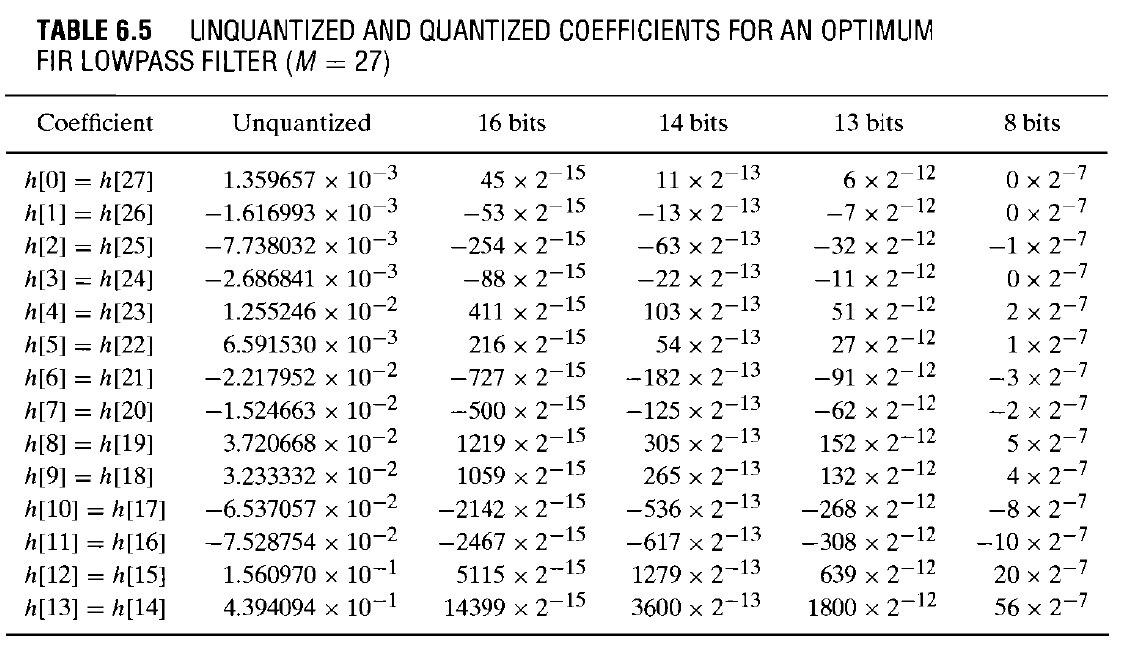
\includegraphics[scale=0.35]{figs/fir_quantized_coefficients.png}
	\end{figure}
	\pause
	\textbf{Question:} will the linear phase property of this FIR filter be preserved after coefficient quantization?
\end{frame}


\begin{frame}{Example: coefficient quantization of linear-phase FIR filter}
	Zeros move around significantly, but they remain in \textbf{conjugate} and \textbf{conjugate reciprocal}  pairs ($\{c, c^*, 1/c, 1/c^*\}$) since symmetry of impulse response is preserved after quantization
	\begin{figure}
		\centering
		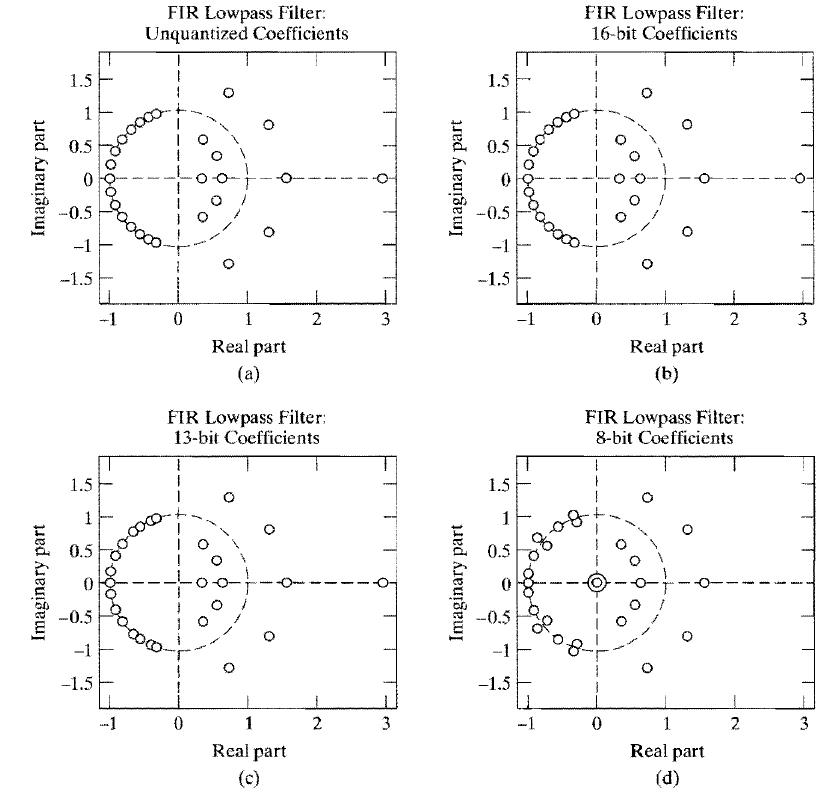
\includegraphics[scale=0.33]{figs/pole_zero_fir_quantized.png}
	\end{figure}
\end{frame}

\begin{frame}{Example: coefficient quantization of linear-phase FIR filter}
	Error in the magnitude response for 13-bit quantization. Error for transition band is not shown.
\begin{center}
		\resizebox{!}{0.8\textheight}{
	\begin{tikzpicture}
		\node (img) {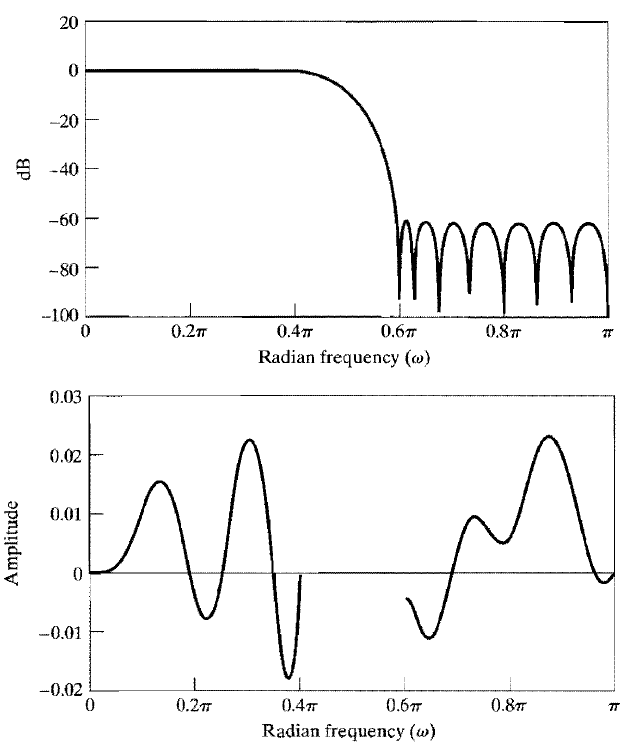
\includegraphics[scale=0.35]{figs/fir_mag_resp_quantized.png}};
		\node[align=center, text width = 2cm, scale=0.8] at ($(img.north east)+(-1.5cm, -1cm)$) {Magnitude response};
		\node[align=center, text width = 4cm, scale=0.8] at ($(img.south east)+(-2.3cm, 3cm)$) {Error after 13-bit coefficient quantization};
	\end{tikzpicture}
	}
\end{center}
\end{frame}

%
\begin{frame}{Example: coefficient quantization in IIR filter}

Bandpass 12th-order elliptic filter
\begin{columns}
\begin{column}{0.5\textwidth}
	\begin{center}
		\resizebox{\textwidth}{!}{\begin{tikzpicture}
\begin{axis}[
axis equal,
axis lines*=middle,
enlargelimits = false, clip=true,
xmin=-1.39,
xmax=1.39,
ymin=-1.10,
ymax=1.10,
axis line style={->,>=stealth},
xlabel={$\mathrm{Re}\{z\}$},
ylabel={$\mathrm{Im}\{z\}$},
every axis x label/.style={
at={(ticklabel* cs:1)},
anchor=north,
},
every axis y label/.style={
at={(ticklabel* cs:1)},
anchor=south,
},
xmajorgrids,
ymajorgrids,
every outer y axis line/.append style={white!15!black},
every y tick label/.append style={font=\color{white!15!black}},
legend style={draw=white!15!black,fill=white,legend cell align=left}]
\draw (axis cs:0,0) circle [black!50, dashed, line width=2pt, radius=1];
\addplot [line width=1pt,mark=x, only marks, mark size = 3pt]
table[row sep=crcr]{
	0.30259 0.94453 \\
	0.30259 -0.94453 \\
	0.31472 0.91236 \\
	0.31472 -0.91236 \\
	0.3692 0.84529 \\
	0.3692 -0.84529 \\
	0.58654 0.80134 \\
	0.58654 -0.80134 \\
	0.55823 0.79298 \\
	0.55823 -0.79298 \\
	0.48019 0.79336 \\
	0.48019 -0.79336 \\
};

\addplot [line width=1pt,mark=*, only marks, mark size = 3pt, mark options={fill=white}]
table[row sep=crcr]{
	-0.096674 0.99532 \\
	-0.096674 -0.99532 \\
	0.23261 0.97257 \\
	0.23261 -0.97257 \\
	0.27546 0.96131 \\
	0.27546 -0.96131 \\
	0.79688 0.60414 \\
	0.79688 -0.60414 \\
	0.63915 0.76908 \\
	0.63915 -0.76908 \\
	0.61128 0.79142 \\
	0.61128 -0.79142 \\
};

\end{axis}
\end{tikzpicture}}
	\end{center}
\end{column}

\begin{column}{0.6\textwidth}
	\begin{center}
		\resizebox{\textwidth}{!}{\begin{tikzpicture}
\begin{axis}[
axis lines*=middle,
enlargelimits = true, clip=true,
scale only axis,
axis line style={->,>=stealth},
%width=0.6\textwidth,
%height=0.4\textwidth,
xlabel={$\omega$},
ylabel={$20\cdot\log_{10}(|H(e^{j\omega})|)$},
every axis x label/.style={
	at={(ticklabel* cs:1)},
	xshift=-0.2cm,
	anchor=north,
},
every axis y label/.style={
	at={(ticklabel* cs:1)},
	xshift=0.4cm,
	%yshift=0.35cm,
	anchor=south,
},
every outer x axis line/.append style={white!15!black},
every x tick label/.append style={font=\color{white!15!black}},
%xmin=0, xmax=1,
xtick={0, 0.25, 0.5, 0.75, 1},
xticklabels ={$0$, $\pi/4$, $\pi/2$, $3\pi/4$, $\pi$},
ymajorgrids,
every outer y axis line/.append style={white!15!black},
every y tick label/.append style={font=\color{white!15!black}},
legend style={draw=white!15!black,fill=white,legend cell align=left}]
\addplot [color=black, solid, line width=1.5pt, forget plot]
table[row sep=crcr]{
	0 -40.6464 \\
	0.0019531 -40.6468 \\
	0.0039063 -40.648 \\
	0.0058594 -40.65 \\
	0.0078125 -40.6529 \\
	0.0097656 -40.6565 \\
	0.011719 -40.6609 \\
	0.013672 -40.6662 \\
	0.015625 -40.6723 \\
	0.017578 -40.6792 \\
	0.019531 -40.687 \\
	0.021484 -40.6955 \\
	0.023438 -40.705 \\
	0.025391 -40.7153 \\
	0.027344 -40.7265 \\
	0.029297 -40.7385 \\
	0.03125 -40.7514 \\
	0.033203 -40.7653 \\
	0.035156 -40.78 \\
	0.037109 -40.7957 \\
	0.039062 -40.8124 \\
	0.041016 -40.8299 \\
	0.042969 -40.8485 \\
	0.044922 -40.8681 \\
	0.046875 -40.8887 \\
	0.048828 -40.9103 \\
	0.050781 -40.9329 \\
	0.052734 -40.9567 \\
	0.054688 -40.9816 \\
	0.056641 -41.0076 \\
	0.058594 -41.0347 \\
	0.060547 -41.063 \\
	0.0625 -41.0926 \\
	0.064453 -41.1234 \\
	0.066406 -41.1555 \\
	0.068359 -41.1889 \\
	0.070312 -41.2237 \\
	0.072266 -41.2599 \\
	0.074219 -41.2975 \\
	0.076172 -41.3366 \\
	0.078125 -41.3773 \\
	0.080078 -41.4195 \\
	0.082031 -41.4634 \\
	0.083984 -41.5089 \\
	0.085938 -41.5563 \\
	0.087891 -41.6054 \\
	0.089844 -41.6564 \\
	0.091797 -41.7094 \\
	0.09375 -41.7643 \\
	0.095703 -41.8214 \\
	0.097656 -41.8807 \\
	0.099609 -41.9423 \\
	0.10156 -42.0062 \\
	0.10352 -42.0726 \\
	0.10547 -42.1416 \\
	0.10742 -42.2132 \\
	0.10938 -42.2877 \\
	0.11133 -42.3651 \\
	0.11328 -42.4455 \\
	0.11523 -42.5292 \\
	0.11719 -42.6163 \\
	0.11914 -42.7069 \\
	0.12109 -42.8012 \\
	0.12305 -42.8995 \\
	0.125 -43.0018 \\
	0.12695 -43.1086 \\
	0.12891 -43.2199 \\
	0.13086 -43.336 \\
	0.13281 -43.4573 \\
	0.13477 -43.584 \\
	0.13672 -43.7164 \\
	0.13867 -43.855 \\
	0.14062 -44.0001 \\
	0.14258 -44.1521 \\
	0.14453 -44.3116 \\
	0.14648 -44.479 \\
	0.14844 -44.6548 \\
	0.15039 -44.8398 \\
	0.15234 -45.0347 \\
	0.1543 -45.2401 \\
	0.15625 -45.457 \\
	0.1582 -45.6863 \\
	0.16016 -45.9291 \\
	0.16211 -46.1866 \\
	0.16406 -46.4603 \\
	0.16602 -46.7517 \\
	0.16797 -47.0627 \\
	0.16992 -47.3954 \\
	0.17188 -47.7522 \\
	0.17383 -48.1361 \\
	0.17578 -48.5505 \\
	0.17773 -48.9995 \\
	0.17969 -49.4881 \\
	0.18164 -50.0224 \\
	0.18359 -50.61 \\
	0.18555 -51.2607 \\
	0.1875 -51.9867 \\
	0.18945 -52.8049 \\
	0.19141 -53.7376 \\
	0.19336 -54.8171 \\
	0.19531 -56.091 \\
	0.19727 -57.6343 \\
	0.19922 -59.5766 \\
	0.20117 -62.1706 \\
	0.20312 -66.0266 \\
	0.20508 -73.4684 \\
	0.20703 -81.527 \\
	0.20898 -68.2129 \\
	0.21094 -63.0763 \\
	0.21289 -59.7955 \\
	0.21484 -57.3632 \\
	0.2168 -55.4199 \\
	0.21875 -53.7957 \\
	0.2207 -52.3967 \\
	0.22266 -51.1657 \\
	0.22461 -50.0655 \\
	0.22656 -49.0702 \\
	0.22852 -48.1618 \\
	0.23047 -47.3267 \\
	0.23242 -46.5552 \\
	0.23437 -45.8397 \\
	0.23633 -45.1747 \\
	0.23828 -44.556 \\
	0.24023 -43.9807 \\
	0.24219 -43.4468 \\
	0.24414 -42.9535 \\
	0.24609 -42.5006 \\
	0.24805 -42.0889 \\
	0.25 -41.7204 \\
	0.25195 -41.3978 \\
	0.25391 -41.1255 \\
	0.25586 -40.9094 \\
	0.25781 -40.7576 \\
	0.25977 -40.6812 \\
	0.26172 -40.6951 \\
	0.26367 -40.8205 \\
	0.26563 -41.0873 \\
	0.26758 -41.5397 \\
	0.26953 -42.2467 \\
	0.27148 -43.3234 \\
	0.27344 -44.9845 \\
	0.27539 -47.7066 \\
	0.27734 -52.9955 \\
	0.2793 -98.5105 \\
	0.28125 -51.7145 \\
	0.2832 -45.426 \\
	0.28516 -42.0675 \\
	0.28711 -40.6874 \\
	0.28906 -42.737 \\
	0.29102 -50.7879 \\
	0.29297 -29.4892 \\
	0.29492 -18.5636 \\
	0.29688 -9.0593 \\
	0.29883 -1.6449 \\
	0.30078 0.072287 \\
	0.30273 -0.070458 \\
	0.30469 -0.06096 \\
	0.30664 0.029322 \\
	0.30859 0.074477 \\
	0.31055 0.056259 \\
	0.3125 0.0050839 \\
	0.31445 -0.046121 \\
	0.31641 -0.077964 \\
	0.31836 -0.084487 \\
	0.32031 -0.068592 \\
	0.32227 -0.037683 \\
	0.32422 -0.00054383 \\
	0.32617 0.034689 \\
	0.32813 0.061736 \\
	0.33008 0.076751 \\
	0.33203 0.078413 \\
	0.33398 0.067617 \\
	0.33594 0.046932 \\
	0.33789 0.019959 \\
	0.33984 -0.0093057 \\
	0.3418 -0.036994 \\
	0.34375 -0.059764 \\
	0.3457 -0.075069 \\
	0.34766 -0.081304 \\
	0.34961 -0.07788 \\
	0.35156 -0.065226 \\
	0.35352 -0.044737 \\
	0.35547 -0.018679 \\
	0.35742 0.0099842 \\
	0.35938 0.037822 \\
	0.36133 0.061261 \\
	0.36328 0.076991 \\
	0.36523 0.082417 \\
	0.36719 0.076126 \\
	0.36914 0.058278 \\
	0.37109 0.030853 \\
	0.37305 -0.0023266 \\
	0.375 -0.035848 \\
	0.37695 -0.063266 \\
	0.37891 -0.077998 \\
	0.38086 -0.074619 \\
	0.38281 -0.050642 \\
	0.38477 -0.0088222 \\
	0.38672 0.040379 \\
	0.38867 0.077638 \\
	0.39063 0.078587 \\
	0.39258 0.028336 \\
	0.39453 -0.050396 \\
	0.39648 -0.069947 \\
	0.39844 0.057742 \\
	0.40039 -0.30328 \\
	0.40234 -4.158 \\
	0.4043 -11.4364 \\
	0.40625 -19.5133 \\
	0.4082 -28.592 \\
	0.41016 -42.2402 \\
	0.41211 -46.9602 \\
	0.41406 -41.2054 \\
	0.41602 -40.775 \\
	0.41797 -42.0992 \\
	0.41992 -44.6663 \\
	0.42188 -48.7922 \\
	0.42383 -56.5839 \\
	0.42578 -66.1767 \\
	0.42773 -53.0138 \\
	0.42969 -48.5452 \\
	0.43164 -46.0027 \\
	0.43359 -44.3403 \\
	0.43555 -43.1844 \\
	0.4375 -42.3572 \\
	0.43945 -41.7597 \\
	0.44141 -41.3314 \\
	0.44336 -41.0322 \\
	0.44531 -40.8346 \\
	0.44727 -40.7188 \\
	0.44922 -40.6701 \\
	0.45117 -40.6777 \\
	0.45312 -40.7328 \\
	0.45508 -40.8288 \\
	0.45703 -40.9606 \\
	0.45898 -41.1239 \\
	0.46094 -41.3153 \\
	0.46289 -41.5321 \\
	0.46484 -41.7722 \\
	0.4668 -42.0339 \\
	0.46875 -42.3158 \\
	0.4707 -42.6168 \\
	0.47266 -42.9363 \\
	0.47461 -43.2737 \\
	0.47656 -43.6287 \\
	0.47852 -44.0011 \\
	0.48047 -44.3912 \\
	0.48242 -44.7992 \\
	0.48438 -45.2255 \\
	0.48633 -45.671 \\
	0.48828 -46.1365 \\
	0.49023 -46.6233 \\
	0.49219 -47.1327 \\
	0.49414 -47.6665 \\
	0.49609 -48.227 \\
	0.49805 -48.8167 \\
	0.5 -49.4387 \\
	0.50195 -50.097 \\
	0.50391 -50.7962 \\
	0.50586 -51.5422 \\
	0.50781 -52.3423 \\
	0.50977 -53.2059 \\
	0.51172 -54.145 \\
	0.51367 -55.1759 \\
	0.51563 -56.3206 \\
	0.51758 -57.6101 \\
	0.51953 -59.0909 \\
	0.52148 -60.8357 \\
	0.52344 -62.9693 \\
	0.52539 -65.7331 \\
	0.52734 -69.7002 \\
	0.5293 -76.9609 \\
	0.53125 -88.0526 \\
	0.5332 -73.2658 \\
	0.53516 -68.1597 \\
	0.53711 -65.0234 \\
	0.53906 -62.7677 \\
	0.54102 -61.0137 \\
	0.54297 -59.5841 \\
	0.54492 -58.3816 \\
	0.54688 -57.347 \\
	0.54883 -56.4414 \\
	0.55078 -55.6383 \\
	0.55273 -54.9183 \\
	0.55469 -54.2671 \\
	0.55664 -53.6739 \\
	0.55859 -53.13 \\
	0.56055 -52.6287 \\
	0.5625 -52.1645 \\
	0.56445 -51.733 \\
	0.56641 -51.3303 \\
	0.56836 -50.9533 \\
	0.57031 -50.5993 \\
	0.57227 -50.2662 \\
	0.57422 -49.9519 \\
	0.57617 -49.6546 \\
	0.57813 -49.373 \\
	0.58008 -49.1058 \\
	0.58203 -48.8517 \\
	0.58398 -48.6097 \\
	0.58594 -48.379 \\
	0.58789 -48.1587 \\
	0.58984 -47.9481 \\
	0.5918 -47.7465 \\
	0.59375 -47.5533 \\
	0.5957 -47.368 \\
	0.59766 -47.1901 \\
	0.59961 -47.0192 \\
	0.60156 -46.8547 \\
	0.60352 -46.6964 \\
	0.60547 -46.5439 \\
	0.60742 -46.3969 \\
	0.60937 -46.2551 \\
	0.61133 -46.1181 \\
	0.61328 -45.9858 \\
	0.61523 -45.858 \\
	0.61719 -45.7343 \\
	0.61914 -45.6146 \\
	0.62109 -45.4987 \\
	0.62305 -45.3865 \\
	0.625 -45.2777 \\
	0.62695 -45.1722 \\
	0.62891 -45.0698 \\
	0.63086 -44.9705 \\
	0.63281 -44.874 \\
	0.63477 -44.7803 \\
	0.63672 -44.6893 \\
	0.63867 -44.6008 \\
	0.64063 -44.5147 \\
	0.64258 -44.431 \\
	0.64453 -44.3495 \\
	0.64648 -44.2702 \\
	0.64844 -44.1929 \\
	0.65039 -44.1177 \\
	0.65234 -44.0444 \\
	0.6543 -43.973 \\
	0.65625 -43.9033 \\
	0.6582 -43.8354 \\
	0.66016 -43.7691 \\
	0.66211 -43.7045 \\
	0.66406 -43.6414 \\
	0.66602 -43.5798 \\
	0.66797 -43.5197 \\
	0.66992 -43.461 \\
	0.67188 -43.4036 \\
	0.67383 -43.3476 \\
	0.67578 -43.2928 \\
	0.67773 -43.2393 \\
	0.67969 -43.187 \\
	0.68164 -43.1358 \\
	0.68359 -43.0857 \\
	0.68555 -43.0368 \\
	0.6875 -42.9889 \\
	0.68945 -42.942 \\
	0.69141 -42.8961 \\
	0.69336 -42.8512 \\
	0.69531 -42.8073 \\
	0.69727 -42.7642 \\
	0.69922 -42.7221 \\
	0.70117 -42.6808 \\
	0.70313 -42.6403 \\
	0.70508 -42.6007 \\
	0.70703 -42.5619 \\
	0.70898 -42.5238 \\
	0.71094 -42.4865 \\
	0.71289 -42.45 \\
	0.71484 -42.4141 \\
	0.7168 -42.379 \\
	0.71875 -42.3445 \\
	0.7207 -42.3107 \\
	0.72266 -42.2776 \\
	0.72461 -42.2451 \\
	0.72656 -42.2132 \\
	0.72852 -42.1819 \\
	0.73047 -42.1512 \\
	0.73242 -42.1211 \\
	0.73438 -42.0915 \\
	0.73633 -42.0625 \\
	0.73828 -42.034 \\
	0.74023 -42.006 \\
	0.74219 -41.9786 \\
	0.74414 -41.9516 \\
	0.74609 -41.9252 \\
	0.74805 -41.8992 \\
	0.75 -41.8737 \\
	0.75195 -41.8486 \\
	0.75391 -41.824 \\
	0.75586 -41.7998 \\
	0.75781 -41.7761 \\
	0.75977 -41.7528 \\
	0.76172 -41.7298 \\
	0.76367 -41.7073 \\
	0.76563 -41.6852 \\
	0.76758 -41.6635 \\
	0.76953 -41.6421 \\
	0.77148 -41.6212 \\
	0.77344 -41.6006 \\
	0.77539 -41.5803 \\
	0.77734 -41.5604 \\
	0.7793 -41.5408 \\
	0.78125 -41.5216 \\
	0.7832 -41.5027 \\
	0.78516 -41.4841 \\
	0.78711 -41.4659 \\
	0.78906 -41.448 \\
	0.79102 -41.4303 \\
	0.79297 -41.413 \\
	0.79492 -41.396 \\
	0.79688 -41.3792 \\
	0.79883 -41.3628 \\
	0.80078 -41.3466 \\
	0.80273 -41.3307 \\
	0.80469 -41.3151 \\
	0.80664 -41.2997 \\
	0.80859 -41.2846 \\
	0.81055 -41.2698 \\
	0.8125 -41.2552 \\
	0.81445 -41.2409 \\
	0.81641 -41.2268 \\
	0.81836 -41.2129 \\
	0.82031 -41.1993 \\
	0.82227 -41.1859 \\
	0.82422 -41.1728 \\
	0.82617 -41.1599 \\
	0.82813 -41.1472 \\
	0.83008 -41.1347 \\
	0.83203 -41.1225 \\
	0.83398 -41.1104 \\
	0.83594 -41.0986 \\
	0.83789 -41.087 \\
	0.83984 -41.0755 \\
	0.8418 -41.0643 \\
	0.84375 -41.0533 \\
	0.8457 -41.0425 \\
	0.84766 -41.0319 \\
	0.84961 -41.0214 \\
	0.85156 -41.0112 \\
	0.85352 -41.0011 \\
	0.85547 -40.9912 \\
	0.85742 -40.9815 \\
	0.85937 -40.972 \\
	0.86133 -40.9627 \\
	0.86328 -40.9535 \\
	0.86523 -40.9445 \\
	0.86719 -40.9357 \\
	0.86914 -40.9271 \\
	0.87109 -40.9186 \\
	0.87305 -40.9102 \\
	0.875 -40.9021 \\
	0.87695 -40.8941 \\
	0.87891 -40.8862 \\
	0.88086 -40.8785 \\
	0.88281 -40.871 \\
	0.88477 -40.8636 \\
	0.88672 -40.8564 \\
	0.88867 -40.8493 \\
	0.89063 -40.8424 \\
	0.89258 -40.8356 \\
	0.89453 -40.829 \\
	0.89648 -40.8225 \\
	0.89844 -40.8162 \\
	0.90039 -40.81 \\
	0.90234 -40.8039 \\
	0.9043 -40.798 \\
	0.90625 -40.7922 \\
	0.9082 -40.7866 \\
	0.91016 -40.781 \\
	0.91211 -40.7757 \\
	0.91406 -40.7704 \\
	0.91602 -40.7653 \\
	0.91797 -40.7603 \\
	0.91992 -40.7555 \\
	0.92188 -40.7508 \\
	0.92383 -40.7462 \\
	0.92578 -40.7417 \\
	0.92773 -40.7374 \\
	0.92969 -40.7332 \\
	0.93164 -40.7291 \\
	0.93359 -40.7251 \\
	0.93555 -40.7213 \\
	0.9375 -40.7176 \\
	0.93945 -40.714 \\
	0.94141 -40.7105 \\
	0.94336 -40.7071 \\
	0.94531 -40.7039 \\
	0.94727 -40.7008 \\
	0.94922 -40.6978 \\
	0.95117 -40.6949 \\
	0.95312 -40.6921 \\
	0.95508 -40.6895 \\
	0.95703 -40.687 \\
	0.95898 -40.6846 \\
	0.96094 -40.6823 \\
	0.96289 -40.6801 \\
	0.96484 -40.678 \\
	0.9668 -40.676 \\
	0.96875 -40.6742 \\
	0.9707 -40.6725 \\
	0.97266 -40.6709 \\
	0.97461 -40.6694 \\
	0.97656 -40.668 \\
	0.97852 -40.6667 \\
	0.98047 -40.6655 \\
	0.98242 -40.6645 \\
	0.98437 -40.6635 \\
	0.98633 -40.6627 \\
	0.98828 -40.662 \\
	0.99023 -40.6614 \\
	0.99219 -40.6609 \\
	0.99414 -40.6605 \\
	0.99609 -40.6602 \\
	0.99805 -40.66 \\
};

\end{axis}
\end{tikzpicture}}
	\end{center}
\end{column}
\end{columns}
\end{frame}

\begin{frame}{Example: coefficient quantization in IIR filter}	
Quantization with 16 bits makes the system \textbf{unstable}. Some of the poles fall outside the unit circle.
\begin{center}
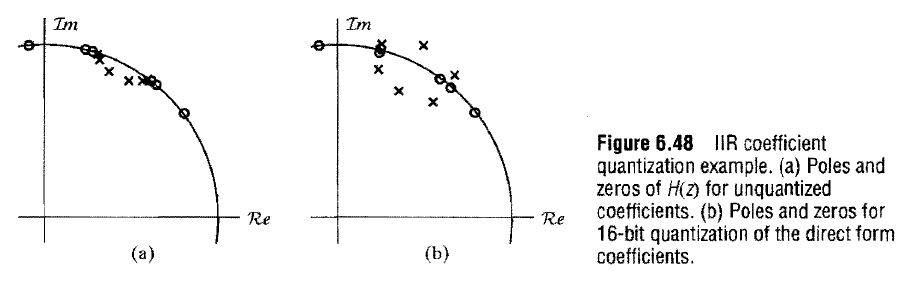
\includegraphics[width=\textwidth]{figs/iir_coeff_quantiz.png}
\end{center}	

\pause
In general, tightly clustered roots are very sensitive to coefficient quantization.

How to mitigate this problem?
\begin{itemize}
\item Higher resolution
\item Cascade or parallel forms are much less sensitive to coefficient quantization than direct forms.
\end{itemize}
\end{frame}


\begin{frame}{Summary on coefficient quantization}
\begin{block}{FIR}
	\begin{itemize}
		\item FIR systems will remain stable after coefficients quantization since all poles are at $z = 0$.
		\item We can preserve the linear phase property by keeping the impulse response symmetric: $h[n] = \pm h[M-n]$. This is typically assured in the implementation by using the special structure for linear phase FIR systems (lecture 7)
		\item Magnitude response is affected, but difference is typically not significant.
	\end{itemize}
\end{block}

\begin{block}{IIR}
	\begin{itemize}
		\item IIR systems can become unstable after coefficients quantization
		\item Symmetry conditions are not easy to enforce. In all-pass systems, for  instance, after quantization the pole $c$ may not longer be conjugate reciprocal of the zero $1/c^*$
		\item These issues are mitigated by increasing word length, or using cascade or parallel forms.
	\end{itemize}
\end{block}

\end{frame}

%
\section{Roundoff Noise}
\begin{frame}{Roundoff noise and the linear noise model}
As for quantization, we'll model roundoff noise as noise source of a \textbf{white uniformly distributed noise} that is independent of the input signal. 

\begin{center}
\resizebox{0.6\textwidth}{!}{\begin{tikzpicture}[->, >=stealth, shorten >= 0pt, draw=black!50, node distance=3.2cm, font=\sffamily]
    \tikzstyle{node}=[circle,fill=black,minimum size=2pt,inner sep=0pt]
    \tikzstyle{block}=[draw=black,rectangle,fill=none,minimum size=1.5cm, inner sep=0pt]
    \tikzstyle{adder}=[draw=black,circle,fill=none,minimum size=1cm, inner sep=0pt]

	\node[node] (xc) {};
    \node[block, right=1.5cm of xc] (Q) {$Q$};
	\coordinate[right=1.5cm of Q] (yc) {};
		
    \path (xc) edge (Q);
    \path (Q) edge (yc);
    
    \node[above = 0mm of xc, text width = 1cm, align=center] {$x[n]$};
    \node[above = 0mm of yc, text width = 3cm, align=center] {$x_Q[n] = Q(x[n])$}; 
	
	\node[node, below=1.5cm of xc] (xc2) {};
	\node[adder] (Q2) at (Q |- xc2) {\Large $+$};
	\coordinate (yc2) at (yc |- Q2) {};
	\node[node, below=1cm of Q2] (e) {};	

 	\path (xc2) edge (Q2);
	\path (Q2) edge (yc2);
	\path (e) edge (Q2);
	
	\node[above = 0mm of xc2, text width = 1cm, align=center] {$x[n]$};
	\node[right = 0mm of e, text width = 3cm, align=center] {$e[n] \sim\mathcal{U}\Big[-\frac{\Delta}{2}, \frac{\Delta}{2}\Big]$};
	\node[above = 0mm of yc2, text width = 3cm, align=center] {$x_Q[n] = x[n] + e[n]$}; 
\end{tikzpicture}}
\end{center}

Assuming $X_m = 1$ (typical), we have the following values:
\begin{align*}
\sigma_B^2 &= \frac{\Delta^2}{12} =  \frac{2^{-2B}}{12}\tag{average power} \\
\phi_{ee}[m] &= \sigma_B^2\delta[m] \tag{autocorrelation function} \\
\Phi_{ee}(e^{j\omega}) &= \sigma_B^2 \tag{PSD}
\end{align*}
\end{frame}

\subsection{Roundoff Noise in FIR Systems}
\begin{frame}{Roundoff noise in FIR systems}
	Direct form of FIR filter
	\begin{center}
		\resizebox{0.75\textwidth}{!}{\begin{tikzpicture}[node distance=1.75cm]
%Place the nodes
\node[terminal={below}{$x[n]$}] (x) at (0,0) {};
\node[terminal={below}{}, right of=x] (00) {};
\node[terminal={below}{}, right of= 00] (01) {};
\node[terminal={below}{}, right of=01] (02) {};
\node[terminal={below}{}, right of=02] (03) {};
\node[terminal={below}{}, right of=03] (04) {};

\coordinate[below of=00] (10) {};
\node[terminal={below}{}, right of=10] (11) {};
\node[terminal={below}{}, right of=11] (12) {};
\node[terminal={below}{}, right of=12] (13) {};
\node[terminal={below}{}, right of=13] (14) {};
\node[terminal={below}{$y[n]$}, right of=14] (y) {};

\foreach \l [count=\j]  in {$h[0]$, $h[1]$, $h[2]$, $h[M-1]$} {
	\pgfmathtruncatemacro{\jn}{(\j-1)}%
	\ifthenelse{\j = 3}
		{\draw[\thickness, dashed] (0\jn) to (0\j)}
		{\draw[zpath={above}] (0\jn) to (0\j)};
	\ifthenelse{\j = 3}
		{\draw[\thickness, dashed] (1\jn) to (1\j)}
		{\draw[amark={}{right}] (1\jn) to (1\j)};
	%\draw[zpath={above}] (0\jn) to (0\j);
	\draw[amark={\l}{right}] (0\jn) to (1\jn);
	
}

\draw[amark={$h[M]$}{right}] (04) to (14);
\draw[amark={}{right}] (14) to (y);

\draw[amark] (x) to (00);
\draw[amark] (14) to (y);

\end{tikzpicture}}
	\end{center}
	\vspace{-0.4cm}
	Two forms of implementation:
	\begin{enumerate}
		\item Quantization immediately after each multiplication:
		\begin{equation*}
		H(z) = \sum_{k = 0}^M Q_B\{h[k]z^{-k}\}
		\end{equation*}
		The multiplication produces $2B+1$ bits, but the $B$ LSBs are discarded.
		\item Quantization immediately after accumulation:
		\begin{equation*}
		H(z) = Q_B\bigg\lbrace\sum_{k = 0}^M h[k]z^{-k}\bigg\rbrace
		\end{equation*}
		Requires ($2B+1$)-bit accumulators (adders). Multiply and accumulate (MAC) instruction in many architectures.
	\end{enumerate}	
\end{frame}


\begin{frame}{1. Quantization immediately after multiplication}
	\begin{center}
		\def\Quantiz{1}
		\resizebox{\textwidth}{!}{\begin{tikzpicture}[node distance=1.75cm]
\tikzstyle{block}=[draw=black,rectangle,fill=none,minimum size=0.2cm, inner sep=2pt, scale=0.75]
\tikzstyle{node}=[red2, circle,fill=red2,minimum size=2pt,inner sep=0pt]

\node[terminal={below}{$x[n]$}] (x) at (0,0) {};
\node[terminal={below}{}, right of=x] (00) {};
\node[terminal={below}{}, right of= 00] (01) {};
\node[terminal={below}{}, right of=01] (02) {};
\node[terminal={below}{}, right of=02] (03) {};
\node[terminal={below}{}, right of=03] (04) {};

\node[terminal={below}{}, below of=00] (10) {};
\node[terminal={below}{}, right of=10] (11) {};
\node[terminal={below}{}, right of=11] (12) {};
\node[terminal={below}{}, right of=12] (13) {};
\node[terminal={below}{}, right of=13] (14) {};
\node[terminal={below}{$\hat{y}[n]$}, right of=14] (y) {};

\if\Quantiz1
	\node[block] (Q0) at ($(00)!0.8!(10)$)  {$Q_B\{\cdot\}$};
	\node[block] (Q1) at ($(01)!0.8!(11)$)  {$Q_B\{\cdot\}$};
	\node[block] (Q2) at ($(02)!0.8!(12)$)  {$Q_B\{\cdot\}$};
	\node[block] (Q3) at ($(03)!0.8!(13)$)  {$Q_B\{\cdot\}$};
	\node[block] (Q4) at ($(04)!0.8!(14)$)  {$Q_B\{\cdot\}$};
	\draw[amark={}{right}] (14) to (y);
\else\relax
	\only<1|handout:1>{
	\node[node, below=1cm of 10] (E0) {}; \node[right, red2] at (E0) {$e_0[n]$};
	\node[node, below=1cm of 11] (E1) {}; \node[right, red2] at (E1) {$e_1[n]$};
	\node[node, below=1cm of 12] (E2) {}; \node[right, red2] at (E2) {$e_2[n]$};
	\node[node, below=1cm of 13] (E3) {}; \node[right, red2] at (E3) {$e_{M-1}[n]$};
	\node[node, below=1cm of 14] (E4) {}; \node[right, red2] at (E4) {$e_{M}[n]$};
	
	\draw[->, >=stealth, red2, \thickness] (E0) to (10);
	\draw[->, >=stealth, red2, \thickness] (E1) to (11);
	\draw[->, >=stealth, red2, \thickness] (E2) to (12);
	\draw[->, >=stealth, red2, \thickness] (E3) to (13);
	\draw[->, >=stealth, red2, \thickness] (E4) to (14);
	\draw[amark={}{right}] (14) to (y);
	}
	\only<2|handout:2>{
		\node[terminal={above}{$y[n]$}] (y2) at ($(14)!0.5!(y)$) {};
		\node[node, below=1cm of y2] (E4) {}; \node[right, red2] at (E4) {$e[n]$};
		\draw[->, >=stealth, red2, \thickness] (E4) to (y2);
		\draw[amark] (y2) to (y);
		\draw[amark] (14) to (y2);
	}
\fi

\foreach \l [count=\j]  in {$h[0]$, $h[1]$, $h[2]$, $h[M-1]$} {
	\pgfmathtruncatemacro{\jn}{(\j-1)}%
	\ifthenelse{\j = 3}
		{\draw[\thickness, dashed] (0\jn) to (0\j)}
		{\draw[zpath={above}] (0\jn) to (0\j)};
	\ifthenelse{\j = 3}
		{\draw[\thickness, dashed] (1\jn) to (1\j)}
		{\draw[amark={}{right}] (1\jn) to (1\j)};
	%\draw[zpath={above}] (0\jn) to (0\j);
	\ifthenelse{\Quantiz = 1}
		{\draw[amark={\l}{right}] (0\jn) to (Q\jn) to (1\jn);}
		{\draw[amark={\l}{right}] (0\jn) to (1\jn);}
}

\if\Quantiz1
	\draw[amark={$h[M]$}{right}] (04) to (Q4) to (14);
\else
	\draw[amark={$h[M]$}{right}] (04) to (14);
\fi
	


\draw[amark] (x) to (00);

\end{tikzpicture}}
	\end{center}

	Equivalent \textbf{linear noise model}:
	
	\only<1|handout:1>{Every noise source has average power: $\sigma_B^2 = \frac{\Delta^2}{12}$}
	\only<2|handout:2>{Lump noise sources into one with average power:  $\E(e^2[n]) = (M+1)\sigma_B^2$}
	\vspace{-0.25cm}
	\begin{center}
		\def\Quantiz{0}
		\resizebox{\textwidth}{!}{\begin{tikzpicture}[node distance=1.75cm]
\tikzstyle{block}=[draw=black,rectangle,fill=none,minimum size=0.2cm, inner sep=2pt, scale=0.75]
\tikzstyle{node}=[red2, circle,fill=red2,minimum size=2pt,inner sep=0pt]

\node[terminal={below}{$x[n]$}] (x) at (0,0) {};
\node[terminal={below}{}, right of=x] (00) {};
\node[terminal={below}{}, right of= 00] (01) {};
\node[terminal={below}{}, right of=01] (02) {};
\node[terminal={below}{}, right of=02] (03) {};
\node[terminal={below}{}, right of=03] (04) {};

\node[terminal={below}{}, below of=00] (10) {};
\node[terminal={below}{}, right of=10] (11) {};
\node[terminal={below}{}, right of=11] (12) {};
\node[terminal={below}{}, right of=12] (13) {};
\node[terminal={below}{}, right of=13] (14) {};
\node[terminal={below}{$\hat{y}[n]$}, right of=14] (y) {};

\if\Quantiz1
	\node[block] (Q0) at ($(00)!0.8!(10)$)  {$Q_B\{\cdot\}$};
	\node[block] (Q1) at ($(01)!0.8!(11)$)  {$Q_B\{\cdot\}$};
	\node[block] (Q2) at ($(02)!0.8!(12)$)  {$Q_B\{\cdot\}$};
	\node[block] (Q3) at ($(03)!0.8!(13)$)  {$Q_B\{\cdot\}$};
	\node[block] (Q4) at ($(04)!0.8!(14)$)  {$Q_B\{\cdot\}$};
	\draw[amark={}{right}] (14) to (y);
\else\relax
	\only<1|handout:1>{
	\node[node, below=1cm of 10] (E0) {}; \node[right, red2] at (E0) {$e_0[n]$};
	\node[node, below=1cm of 11] (E1) {}; \node[right, red2] at (E1) {$e_1[n]$};
	\node[node, below=1cm of 12] (E2) {}; \node[right, red2] at (E2) {$e_2[n]$};
	\node[node, below=1cm of 13] (E3) {}; \node[right, red2] at (E3) {$e_{M-1}[n]$};
	\node[node, below=1cm of 14] (E4) {}; \node[right, red2] at (E4) {$e_{M}[n]$};
	
	\draw[->, >=stealth, red2, \thickness] (E0) to (10);
	\draw[->, >=stealth, red2, \thickness] (E1) to (11);
	\draw[->, >=stealth, red2, \thickness] (E2) to (12);
	\draw[->, >=stealth, red2, \thickness] (E3) to (13);
	\draw[->, >=stealth, red2, \thickness] (E4) to (14);
	\draw[amark={}{right}] (14) to (y);
	}
	\only<2|handout:2>{
		\node[terminal={above}{$y[n]$}] (y2) at ($(14)!0.5!(y)$) {};
		\node[node, below=1cm of y2] (E4) {}; \node[right, red2] at (E4) {$e[n]$};
		\draw[->, >=stealth, red2, \thickness] (E4) to (y2);
		\draw[amark] (y2) to (y);
		\draw[amark] (14) to (y2);
	}
\fi

\foreach \l [count=\j]  in {$h[0]$, $h[1]$, $h[2]$, $h[M-1]$} {
	\pgfmathtruncatemacro{\jn}{(\j-1)}%
	\ifthenelse{\j = 3}
		{\draw[\thickness, dashed] (0\jn) to (0\j)}
		{\draw[zpath={above}] (0\jn) to (0\j)};
	\ifthenelse{\j = 3}
		{\draw[\thickness, dashed] (1\jn) to (1\j)}
		{\draw[amark={}{right}] (1\jn) to (1\j)};
	%\draw[zpath={above}] (0\jn) to (0\j);
	\ifthenelse{\Quantiz = 1}
		{\draw[amark={\l}{right}] (0\jn) to (Q\jn) to (1\jn);}
		{\draw[amark={\l}{right}] (0\jn) to (1\jn);}
}

\if\Quantiz1
	\draw[amark={$h[M]$}{right}] (04) to (Q4) to (14);
\else
	\draw[amark={$h[M]$}{right}] (04) to (14);
\fi
	


\draw[amark] (x) to (00);

\end{tikzpicture}}
	\end{center}
\end{frame}

\begin{frame}{2. Quantization immediately after accumulation}
	\begin{center}
		\def\Quantiz{1}
		\resizebox{\textwidth}{!}{\begin{tikzpicture}[node distance=1.75cm]
\tikzstyle{block}=[draw=black,rectangle,fill=none,minimum size=0.2cm, inner sep=2pt, scale=0.75]
\tikzstyle{node}=[red2, circle,fill=red2,minimum size=2pt,inner sep=0pt]

\node[terminal={below}{$x[n]$}] (x) at (0,0) {};
\node[terminal={below}{}, right of=x] (00) {};
\node[terminal={below}{}, right of= 00] (01) {};
\node[terminal={below}{}, right of=01] (02) {};
\node[terminal={below}{}, right of=02] (03) {};
\node[terminal={below}{}, right of=03] (04) {};

\coordinate[below of=00] (10) {};
\node[terminal={below}{}, right of=10] (11) {};
\node[terminal={below}{}, right of=11] (12) {};
\node[terminal={below}{}, right of=12] (13) {};
\node[terminal={below}{}, right of=13] (14) {};
\node[terminal={below}{$\hat{y}[n]$}, right of=14] (y) {};

\foreach \l [count=\j]  in {$h[0]$, $h[1]$, $h[2]$, $h[M-1]$} {
	\pgfmathtruncatemacro{\jn}{(\j-1)}%
	\ifthenelse{\j = 3}
		{\draw[\thickness, dashed] (0\jn) to (0\j)}
		{\draw[zpath={above}] (0\jn) to (0\j)};
	\ifthenelse{\j = 3}
		{\draw[\thickness, dashed] (1\jn) to (1\j)}
		{\draw[amark={}{right}] (1\jn) to (1\j)};
	%\draw[zpath={above}] (0\jn) to (0\j);
	\draw[amark={\l}{right}] (0\jn) to (1\jn);
	
}

\draw[amark={$h[M]$}{right}] (04) to (14);

\draw[amark] (x) to (00);


\if\Quantiz1
	\node[block] (Q0) at ($(14)!0.5!(y)$)  {$Q_B\{\cdot\}$};
	\draw[amark] (14) to (Q0);
	\draw[amark] (Q0) to (y);
\else
	\node[terminal={above}{$y[n]$}] at ($(14)!0.5!(y)$) (y2) {};
	\draw[amark] (14) to (y2);
	\draw[amark] (y2) to (y);
	
	\node[node, below=1cm of y2] (E4) {}; \node[right, red2] at (E4) {$e[n]$};
	\draw[->, >=stealth, red2, \thickness] (E4) to (y2);
\fi

\end{tikzpicture}}
	\end{center}
	Equivalent \textbf{linear noise model}:
	
	Output noise source has average power $\E(e^2[n]) = \frac{\Delta^2}{12}$. The noise power is ($M+1$) times smaller than in quantization after multiplication
	\vspace{-0.5cm}
	\begin{center}
		\def\Quantiz{0}
		\resizebox{\textwidth}{!}{\begin{tikzpicture}[node distance=1.75cm]
\tikzstyle{block}=[draw=black,rectangle,fill=none,minimum size=0.2cm, inner sep=2pt, scale=0.75]
\tikzstyle{node}=[red2, circle,fill=red2,minimum size=2pt,inner sep=0pt]

\node[terminal={below}{$x[n]$}] (x) at (0,0) {};
\node[terminal={below}{}, right of=x] (00) {};
\node[terminal={below}{}, right of= 00] (01) {};
\node[terminal={below}{}, right of=01] (02) {};
\node[terminal={below}{}, right of=02] (03) {};
\node[terminal={below}{}, right of=03] (04) {};

\coordinate[below of=00] (10) {};
\node[terminal={below}{}, right of=10] (11) {};
\node[terminal={below}{}, right of=11] (12) {};
\node[terminal={below}{}, right of=12] (13) {};
\node[terminal={below}{}, right of=13] (14) {};
\node[terminal={below}{$\hat{y}[n]$}, right of=14] (y) {};

\foreach \l [count=\j]  in {$h[0]$, $h[1]$, $h[2]$, $h[M-1]$} {
	\pgfmathtruncatemacro{\jn}{(\j-1)}%
	\ifthenelse{\j = 3}
		{\draw[\thickness, dashed] (0\jn) to (0\j)}
		{\draw[zpath={above}] (0\jn) to (0\j)};
	\ifthenelse{\j = 3}
		{\draw[\thickness, dashed] (1\jn) to (1\j)}
		{\draw[amark={}{right}] (1\jn) to (1\j)};
	%\draw[zpath={above}] (0\jn) to (0\j);
	\draw[amark={\l}{right}] (0\jn) to (1\jn);
	
}

\draw[amark={$h[M]$}{right}] (04) to (14);

\draw[amark] (x) to (00);


\if\Quantiz1
	\node[block] (Q0) at ($(14)!0.5!(y)$)  {$Q_B\{\cdot\}$};
	\draw[amark] (14) to (Q0);
	\draw[amark] (Q0) to (y);
\else
	\node[terminal={above}{$y[n]$}] at ($(14)!0.5!(y)$) (y2) {};
	\draw[amark] (14) to (y2);
	\draw[amark] (y2) to (y);
	
	\node[node, below=1cm of y2] (E4) {}; \node[right, red2] at (E4) {$e[n]$};
	\draw[->, >=stealth, red2, \thickness] (E4) to (y2);
\fi

\end{tikzpicture}}
	\end{center}
\end{frame}

\begin{frame}{Preventing overflow in FIR systems}
	Larger range $X_m$ reduces chance of overflow, but leads to higher quantization error.
	 \begin{center}
		\resizebox{0.9\textwidth}{!}{\begin{tikzpicture}
	\tikzstyle{node}=[circle,draw=black!50,fill=black,minimum size=2pt,inner sep=0pt]
	\tikzstyle{block}=[draw=black,rectangle,fill=none,minimum size=1cm, inner sep=0pt]
	\begin{axis}[
		axis lines*=middle,
		enlargelimits = false, clip=true,
		ymin=-4, ymax=5,
		xmin=-6.5, xmax=6.5,
		width=\textwidth,
		height=0.7\textwidth,
		axis line style={->,>=stealth},
		xlabel={$x$},
		ylabel={$x_B = Q_B(x)$},
		yticklabel style = {yshift=0.2cm},
		xticklabel style = {yshift=-0.1cm},
		every axis x label/.style={
			at={(ticklabel* cs:1)},
			anchor=west,
		},
		every axis y label/.style={
			at={(ticklabel* cs:1)},
			anchor=south,
		},
		ytick={-4, -3,-2, 1, 2, 3},
		yticklabels={$-4\Delta$, $-3\Delta$, $-2\Delta$, $\Delta$, $2\Delta$, $3\Delta$},
		xtick={-4.5,-3.5,-2.5, 0.5,1.5,...,4.5},
		xticklabels={$-\frac{9\Delta}{2}$, $-\frac{7\Delta}{2}$, $-\frac{5\Delta}{2}$, $\frac{\Delta}{2}$, $\frac{3\Delta}{2}$, $\frac{5\Delta}{2}$, $\frac{7\Delta}{2}$, $\frac{9\Delta}{2}$},
		every outer y axis line/.append style={white!15!black},
		every y tick label/.append style={font=\color{white!15!black}},
		legend style={draw=white!15!black,fill=white,legend cell align=left}]			
		\addplot[line width=1pt] coordinates {(0, 0) (1/2, 0) (1/2, 1) (3/2, 1) (3/2, 2) (5/2, 2) (5/2, 3) (7/2, 3)};
		\addplot[line width=1pt] coordinates {(0, 0) (-1/2, 0) (-1/2, -1) (-3/2, -1) (-3/2, -2) (-5/2, -2) (-5/2, -3) (-7/2, -3) (-7/2, -4) (-9/2, -4)};
	
		\addplot[line width=1pt] coordinates {(7/2, 3) (7/2, -4) (9/2, -4) (9/2, -3) (11/2, -3) (11/2, -2) (13/2, -2) (13/2, -1) (15/2, -1)};
		\addplot[line width=1pt] coordinates {(-9/2, -4) (-9/2, 3) (-11/2, 3) (-11/2, 2) (-13/2, 2) (-13/2, 1) (-15/2, 1)};
	
		%\addplot[dashed, black!20, line width=1pt, domain=-4:4, samples=2] {x};
			
		\foreach \x [count=\cnt] in {100, 101, 110, 111, 000, 001, 010, 011} {
			\edef\temp{\noexpand\node [above, align=center] at (axis cs: \cnt-5,\cnt-5) {$\x$};}
			\temp
			\edef\temp{\noexpand\node [above, align=center] at (axis cs: \cnt+3,\cnt-5) {$\x$};}
			\temp
		}
	
		\node [above, align=center] at (axis cs: -5, 3) {$011$};
		\node [above, align=center] at (axis cs: -6, 2) {$010$};	
		\node [above, align=center] at (axis cs: -7, 1) {$001$};	
			
		\draw[<->, >=stealth, blue2, line width=2pt] (axis cs: -4.5, 0) -- (axis cs: 3.5, 0) {};
		\draw[->, >=stealth, red2, line width=2pt] (axis cs: -4.5, 0) -- (axis cs: -6.5, 0) {};
		\draw[->, >=stealth, red2, line width=2pt] (axis cs: 3.5, 0) -- (axis cs: 6, 0) {};
		\node at (axis cs: 2.5, 0.5) {\color{blue2} $2X_m$};
		\node at (axis cs: 4.5, 0.5) {\color{red2} oveflow};  
		\node at (axis cs: -5.5, 0.5) {\color{red2} oveflow};
	\end{axis}
\end{tikzpicture}}
	\end{center}
\end{frame}

\begin{frame}{Preventing overflow in FIR systems}
	
	Assuming that the input signal is bounded between $-1 \leq x[n] \leq 1$. Overflow will \underline{not} happen, if $|y[n]| < 1$ for any input $x[n]$. 
	
	What are the conditions in the coefficients $h[n]$ to avoid overflow?
	\begin{align*}
		|y[n]| &= \bigg|\sum_{k = 0}^{M} h[k]x[n-k]\bigg| \tag{modulus of convolution sum} \\
		&\leq \sum_{k = 0}^{M} |h[k]|\cdot|x[n-k]| \tag{Schwarz inequality} \\
		&\leq \sum_{k = 0}^{M} |h[k]| \tag{since $-1 \leq x[n] \leq 1$} \\
		& < 1 \implies \text{no overflow}
	\end{align*}
\end{frame}

\subsection{Roundoff Noise in IIR Systems}
\begin{frame}{Roundoff noise in IIR systems}

\begin{itemize}
	\item We'll treat roundoff noise in IIR systems similarly to in FIR systems
	\item The inherent feedback of IIR systems will lead to roundoff noise \textbf{shaping}
	\item Now the difference between the different structures will become apparent
		\begin{itemize}
		\item Direct form I \& II
		\item Transposed forms
		\item Cascade forms
		\item Parallel forms
	\end{itemize}
\end{itemize}
\end{frame}

\begin{frame}{Direct form I IIR filter}
	Quantization is performed after every multiplication
	\begin{center}
		\def\QUANTIZ{1}
		\resizebox{\textwidth}{!}{\begin{tikzpicture}[node distance=1.75cm]
\tikzstyle{block}=[draw=black,rectangle,fill=none,minimum size=0.2cm, inner sep=2pt, scale=0.75]
\tikzstyle{node}=[red2, circle,fill=red2,minimum size=2pt,inner sep=0pt]

\node[terminal={below}{$x[n]$}] (x) at (0,0) {};
\node[terminal={below}{}, right of=x] (00) {};
\node[terminal={below}{}, right=2cm of 00] (01) {};
\node[terminal={below}{}, right of=01] (02) {};
\node[terminal={below}{}, right=2cm of 02] (03) {};
\node[terminal={below}{$y[n]$}, right of=03] (y) {};

\foreach \j in {1, 2} {
	\pgfmathtruncatemacro{\jn}{(\j-1)}%
	\node[terminal={left}{}, below of=\jn0] (\j0) {};
	\node[terminal={left}{}, below of=\jn1] (\j1) {};
	\node[terminal={left}{}, below of=\jn2] (\j2) {};
	\node[terminal={right}{}, below of=\jn3] (\j3) {};
	\draw[amark={$z^{-1}$}{left}] (\jn0) to (\j0);
	\draw[amark={}{left}] (\j1) to (\jn1);
	\draw[amark={}{left}] (\j2) to (\jn2);
	\draw[amark={$z^{-1}$}{right}] (\jn3) to (\j3);
}

\if\QUANTIZ2  % lumped noise sources
	\foreach \j in {0, 1, 2} {		
		\draw[amark={$b_\j$}{above}] (\j0) to (\j1);		
		\ifthenelse{\j = 0}
			{\draw[amark={$1$}{above}] (\j3) to (\j2);}
			{\draw[amark={$a_\j$}{above}] (\j3) to (\j2);}
	}
	\node[node, above=0.5cm of 02] (E) {}; \node[right, red2] at (E) {$e[n]$};
	\draw[->, >=stealth, red2, \thickness] (E) to (02);
	
	\onslide<2|handout:1>{
		\draw[dashed] ($(02)-(0.25cm, -0.5cm)$) rectangle ($(23)+(0.7cm, -0.25cm)$);
	}
	
\else % QUANTIZ = 1 -> Quantizers | QUANTIZ = 0 -> noise sources

	\foreach \j in {0, 1, 2} { %b
		\ifthenelse{\QUANTIZ = 1}
			{\node[block] (Q\j0) at ($(\j0)!0.5!(\j1)$) {$Q_B\{\cdot\}$};}
			{\node[terminal={left}{}] (Q\j0) at ($(\j0)!0.5!(\j1)$) {};}
			
		\draw[amark={$b_\j$}{above}] (\j0) to (Q\j0);
		\draw[amark={}{above}] (Q\j0) to (\j1);
	}

	\draw[amark={$1$}{above}] (03) to (02);
	\foreach \j in {1, 2} { %a
		\ifthenelse{\QUANTIZ = 1}
		{\node[block] (Q\j1) at ($(\j2)!0.5!(\j3)$) {$Q_B\{\cdot\}$};}
		{\node[terminal={left}{}] (Q\j1) at ($(\j2)!0.5!(\j3)$) {};}
			
		\draw[amark={$a_\j$}{above}] (\j3) to (Q\j1);	
		\draw[amark={}{above}] (Q\j1) to (\j2);
	}
	
	\if\QUANTIZ0
		\foreach \j in {0, 1, 2} { % b
			\node[node, above=0.5cm of Q\j0] (E\j0) {}; \node[right, red2] at (E\j0) {$e_{b_\j}[n]$};
			\draw[->, >=stealth, red2, \thickness] (E\j0) to (Q\j0);
		}
	
		\foreach \j in {1, 2} { %a
			\node[node, above=0.5cm of Q\j1] (E\j1) {}; \node[right, red2] at (E\j1) {$e_{a_\j}[n]$};
			\draw[->, >=stealth, red2, \thickness] (E\j1) to (Q\j1);
		}
	\else\relax
	\fi
\fi


\draw[amark={}{right}] (x) to (00);
\draw[amark={}{right}] (01) to (02);
\draw[amark={}{right}] (03) to (y);

\end{tikzpicture}}
	\end{center}
\end{frame}

\begin{frame}{Direct form I IIR filter}
As for FIR filters, we can replace the quantizers by noise sources with average power
\begin{equation*}
\sigma_B^2 = \frac{\Delta^2}{12} = \frac{2^{-2B}}{12}
\end{equation*}
\begin{center}
	\def\QUANTIZ{0}
	\resizebox{\textwidth}{!}{\begin{tikzpicture}[node distance=1.75cm]
\tikzstyle{block}=[draw=black,rectangle,fill=none,minimum size=0.2cm, inner sep=2pt, scale=0.75]
\tikzstyle{node}=[red2, circle,fill=red2,minimum size=2pt,inner sep=0pt]

\node[terminal={below}{$x[n]$}] (x) at (0,0) {};
\node[terminal={below}{}, right of=x] (00) {};
\node[terminal={below}{}, right=2cm of 00] (01) {};
\node[terminal={below}{}, right of=01] (02) {};
\node[terminal={below}{}, right=2cm of 02] (03) {};
\node[terminal={below}{$y[n]$}, right of=03] (y) {};

\foreach \j in {1, 2} {
	\pgfmathtruncatemacro{\jn}{(\j-1)}%
	\node[terminal={left}{}, below of=\jn0] (\j0) {};
	\node[terminal={left}{}, below of=\jn1] (\j1) {};
	\node[terminal={left}{}, below of=\jn2] (\j2) {};
	\node[terminal={right}{}, below of=\jn3] (\j3) {};
	\draw[amark={$z^{-1}$}{left}] (\jn0) to (\j0);
	\draw[amark={}{left}] (\j1) to (\jn1);
	\draw[amark={}{left}] (\j2) to (\jn2);
	\draw[amark={$z^{-1}$}{right}] (\jn3) to (\j3);
}

\if\QUANTIZ2  % lumped noise sources
	\foreach \j in {0, 1, 2} {		
		\draw[amark={$b_\j$}{above}] (\j0) to (\j1);		
		\ifthenelse{\j = 0}
			{\draw[amark={$1$}{above}] (\j3) to (\j2);}
			{\draw[amark={$a_\j$}{above}] (\j3) to (\j2);}
	}
	\node[node, above=0.5cm of 02] (E) {}; \node[right, red2] at (E) {$e[n]$};
	\draw[->, >=stealth, red2, \thickness] (E) to (02);
	
	\onslide<2|handout:1>{
		\draw[dashed] ($(02)-(0.25cm, -0.5cm)$) rectangle ($(23)+(0.7cm, -0.25cm)$);
	}
	
\else % QUANTIZ = 1 -> Quantizers | QUANTIZ = 0 -> noise sources

	\foreach \j in {0, 1, 2} { %b
		\ifthenelse{\QUANTIZ = 1}
			{\node[block] (Q\j0) at ($(\j0)!0.5!(\j1)$) {$Q_B\{\cdot\}$};}
			{\node[terminal={left}{}] (Q\j0) at ($(\j0)!0.5!(\j1)$) {};}
			
		\draw[amark={$b_\j$}{above}] (\j0) to (Q\j0);
		\draw[amark={}{above}] (Q\j0) to (\j1);
	}

	\draw[amark={$1$}{above}] (03) to (02);
	\foreach \j in {1, 2} { %a
		\ifthenelse{\QUANTIZ = 1}
		{\node[block] (Q\j1) at ($(\j2)!0.5!(\j3)$) {$Q_B\{\cdot\}$};}
		{\node[terminal={left}{}] (Q\j1) at ($(\j2)!0.5!(\j3)$) {};}
			
		\draw[amark={$a_\j$}{above}] (\j3) to (Q\j1);	
		\draw[amark={}{above}] (Q\j1) to (\j2);
	}
	
	\if\QUANTIZ0
		\foreach \j in {0, 1, 2} { % b
			\node[node, above=0.5cm of Q\j0] (E\j0) {}; \node[right, red2] at (E\j0) {$e_{b_\j}[n]$};
			\draw[->, >=stealth, red2, \thickness] (E\j0) to (Q\j0);
		}
	
		\foreach \j in {1, 2} { %a
			\node[node, above=0.5cm of Q\j1] (E\j1) {}; \node[right, red2] at (E\j1) {$e_{a_\j}[n]$};
			\draw[->, >=stealth, red2, \thickness] (E\j1) to (Q\j1);
		}
	\else\relax
	\fi
\fi


\draw[amark={}{right}] (x) to (00);
\draw[amark={}{right}] (01) to (02);
\draw[amark={}{right}] (03) to (y);

\end{tikzpicture}}
\end{center}
\end{frame}

\begin{frame}{Direct form I IIR filter}
Combining all noise sources into one
\begin{equation*}
\sigma_e^2 = (M+1+N)\sigma^2_B = (M+1+N)\frac{2^{-2B}}{12}
\end{equation*}
\begin{center}
	\def\QUANTIZ{2}
	\resizebox{\textwidth}{!}{\begin{tikzpicture}[node distance=1.75cm]
\tikzstyle{block}=[draw=black,rectangle,fill=none,minimum size=0.2cm, inner sep=2pt, scale=0.75]
\tikzstyle{node}=[red2, circle,fill=red2,minimum size=2pt,inner sep=0pt]

\node[terminal={below}{$x[n]$}] (x) at (0,0) {};
\node[terminal={below}{}, right of=x] (00) {};
\node[terminal={below}{}, right=2cm of 00] (01) {};
\node[terminal={below}{}, right of=01] (02) {};
\node[terminal={below}{}, right=2cm of 02] (03) {};
\node[terminal={below}{$y[n]$}, right of=03] (y) {};

\foreach \j in {1, 2} {
	\pgfmathtruncatemacro{\jn}{(\j-1)}%
	\node[terminal={left}{}, below of=\jn0] (\j0) {};
	\node[terminal={left}{}, below of=\jn1] (\j1) {};
	\node[terminal={left}{}, below of=\jn2] (\j2) {};
	\node[terminal={right}{}, below of=\jn3] (\j3) {};
	\draw[amark={$z^{-1}$}{left}] (\jn0) to (\j0);
	\draw[amark={}{left}] (\j1) to (\jn1);
	\draw[amark={}{left}] (\j2) to (\jn2);
	\draw[amark={$z^{-1}$}{right}] (\jn3) to (\j3);
}

\if\QUANTIZ2  % lumped noise sources
	\foreach \j in {0, 1, 2} {		
		\draw[amark={$b_\j$}{above}] (\j0) to (\j1);		
		\ifthenelse{\j = 0}
			{\draw[amark={$1$}{above}] (\j3) to (\j2);}
			{\draw[amark={$a_\j$}{above}] (\j3) to (\j2);}
	}
	\node[node, above=0.5cm of 02] (E) {}; \node[right, red2] at (E) {$e[n]$};
	\draw[->, >=stealth, red2, \thickness] (E) to (02);
	
	\onslide<2|handout:1>{
		\draw[dashed] ($(02)-(0.25cm, -0.5cm)$) rectangle ($(23)+(0.7cm, -0.25cm)$);
	}
	
\else % QUANTIZ = 1 -> Quantizers | QUANTIZ = 0 -> noise sources

	\foreach \j in {0, 1, 2} { %b
		\ifthenelse{\QUANTIZ = 1}
			{\node[block] (Q\j0) at ($(\j0)!0.5!(\j1)$) {$Q_B\{\cdot\}$};}
			{\node[terminal={left}{}] (Q\j0) at ($(\j0)!0.5!(\j1)$) {};}
			
		\draw[amark={$b_\j$}{above}] (\j0) to (Q\j0);
		\draw[amark={}{above}] (Q\j0) to (\j1);
	}

	\draw[amark={$1$}{above}] (03) to (02);
	\foreach \j in {1, 2} { %a
		\ifthenelse{\QUANTIZ = 1}
		{\node[block] (Q\j1) at ($(\j2)!0.5!(\j3)$) {$Q_B\{\cdot\}$};}
		{\node[terminal={left}{}] (Q\j1) at ($(\j2)!0.5!(\j3)$) {};}
			
		\draw[amark={$a_\j$}{above}] (\j3) to (Q\j1);	
		\draw[amark={}{above}] (Q\j1) to (\j2);
	}
	
	\if\QUANTIZ0
		\foreach \j in {0, 1, 2} { % b
			\node[node, above=0.5cm of Q\j0] (E\j0) {}; \node[right, red2] at (E\j0) {$e_{b_\j}[n]$};
			\draw[->, >=stealth, red2, \thickness] (E\j0) to (Q\j0);
		}
	
		\foreach \j in {1, 2} { %a
			\node[node, above=0.5cm of Q\j1] (E\j1) {}; \node[right, red2] at (E\j1) {$e_{a_\j}[n]$};
			\draw[->, >=stealth, red2, \thickness] (E\j1) to (Q\j1);
		}
	\else\relax
	\fi
\fi


\draw[amark={}{right}] (x) to (00);
\draw[amark={}{right}] (01) to (02);
\draw[amark={}{right}] (03) to (y);

\end{tikzpicture}}
\end{center}

\onslide<2|handout:1>{Quantization noise is \textbf{shaped} by the filter defined in the dashed rectangle:
\begin{equation*}
H_a(z) = \frac{1}{A(z)} = \frac{1}{1 + a_1z^{-1} + a_2z^{-2}} \tag{shaped by the poles}
\end{equation*}
}
\end{frame}

\begin{frame}{Direct form I IIR filter}
	Calculating the roundoff noise PSD at the output:
	\begin{align*}
	\Phi_{\tilde{e}\tilde{e}}(e^{j\omega}) &= |H_a(e^{j\omega})|^2\Phi_{ee}(e^{j\omega}) \\
	& = \frac{1}{|A(e^{j\omega})|^2}(M+N+1)\sigma_B^2
	\end{align*}
	
	The average power is obtained by integrating the PSD over $[-\pi, \pi]$:
	\begin{align*}
	\sigma_{\tilde{e}}^2 &=\frac{1}{2\pi}\int_{-\pi}^{\pi}\Phi_{\tilde{e}\tilde{e}}(e^{j\omega})d\omega \\
	&=(M+N+1)\frac{\sigma_B^2}{2\pi}\int_{-\pi}^{\pi} \frac{1}{|A(e^{j\omega})|^2}d\omega
	\end{align*}
	
	The actual value will depend on $A(e^{j\omega})$, but the integral could be larger than 1. That is, $A(e^{j\omega})$ could \underline{enhance} the roundoff noise.
	
\end{frame}

%
\begin{frame}{Direct form II IIR filter}
 Similarly to the direct form I, quantization may be performed after multiplications. The quantizers are replaced by noise sources of average power $\sigma_B^2$. Noise sources are combined whenever possible
 
\begin{align*}
\sigma_{e_1}^2 &= N\sigma_B^2 \tag{average power of $e_1[n]$} \\
\sigma_{e_2}^2 &= (M+1)\sigma_B^2 \tag{average power of $e_2[n]$} \\
\end{align*}
 
\begin{center}
	\resizebox{0.7\textwidth}{!}{\begin{tikzpicture}[node distance=1.75cm]
\tikzstyle{node}=[red2, circle,fill=red2,minimum size=2pt,inner sep=0pt]
%Place the nodes
\node[terminal={below}{$x[n]$}] (x) at (0,0) {};
\node[terminal={below}{}, right of=x] (00) {};
\node[terminal={below}{}, right of= 00] (01) {};
\node[terminal={below}{}, right of=01] (02) {};
\node[terminal={below}{$y[n]$}, right of=02] (y) {};

\foreach \j in {1, 2} {
	\pgfmathtruncatemacro{\jn}{(\j-1)}%
	\node[terminal={below}{}, below of=\jn0] (\j0) {};
	\node[terminal={below}{}, below of=\jn1] (\j1) {};
	\node[terminal={below}{}, below of=\jn2] (\j2) {};
}

%
\draw[zpath={right}] (01) to (11);
\draw[zpath={right}] (11) to (21);

%
\draw[amark] (10) to (00);
\draw[amark] (20) to (10);

%
\draw[amark] (12) to (02);
\draw[amark] (22) to (12);

%
\draw[amark={$1$}{above}] (00) to (01);
\draw[amark={$a_1$}{above}] (11) to (10);
\draw[amark={$a_2$}{above}] (21) to (20);

%
\draw[amark={$b_0$}{above}] (01) to (02);
\draw[amark={$b_1$}{above}] (11) to (12);
\draw[amark={$b_2$}{above}] (21) to (22);

\draw[amark] (x) to (00);
\draw[amark] (02) to (y);

\node[node, above=0.5cm of 00] (E1) {}; \node[right, red2] at (E1) {$e_1[n]$};
\node[node, above=0.5cm of 02] (E2) {}; \node[right, red2] at (E2) {$e_2[n]$};
\draw[->, >=stealth, red2, \thickness] (E1) to (00);
\draw[->, >=stealth, red2, \thickness] (E2) to (02);

\end{tikzpicture}}
\end{center}

\end{frame}

\begin{frame}

Noise source $e_2[n]$ is already at the output, but $e_1[n]$ will be shaped by the filter $H(z)$:

\begin{align*}
\Phi_{\tilde{e}\tilde{e}}(e^{j\omega}) &= |H(e^{j\omega})|^2\Phi_{e_1e_1}(e^{j\omega}) +  \Phi_{e_2e_2}(e^{j\omega})\\
& = N\sigma_{B}^2|H(e^{j\omega})|^2 + (M+1)\sigma_{B}^2
\end{align*}

The average quantization noise power at the output is given by
\begin{align*}
\sigma_{\tilde{e}}^2 & =\frac{1}{2\pi}\int_{-\pi}^{\pi}\Phi_{\tilde{e}\tilde{e}}(e^{j\omega})d\omega \\
&= N\sigma_{B}^2\frac{1}{2\pi}\int_{-\pi}^{\pi} |H(e^{j\omega})|^2d\omega + (M+1)\sigma_{B}^2 \\
&= N\sigma_{B}^2\sum_{n=-\infty}^{\infty}|h[n]|^2 + (M+1)\sigma_{B}^2
\end{align*}

\end{frame}

\begin{frame}{What about transposed forms?}
	\begin{columns}[t]
		\begin{column}{0.5\textwidth}
			\textbf{Transposed direct form I}
			\begin{center}
				\resizebox{1.2\textwidth}{!}{\begin{tikzpicture}[node distance=1.75cm]
\tikzstyle{block}=[draw=black,rectangle,fill=none,minimum size=0.2cm, inner sep=2pt, scale=0.75]
\tikzstyle{node}=[red2, circle,fill=red2,minimum size=2pt,inner sep=0pt]

\node[terminal={below}{$x[n]$}] (x) at (0,0) {};
\node[terminal={below}{}, right of=x] (00) {};
\node[terminal={below}{}, right=2cm of 00] (01) {};
\node[terminal={below}{}, right of=01] (02) {};
\node[terminal={below}{}, right=2cm of 02] (03) {};
\node[terminal={below}{$y[n]$}, right of=03] (y) {};

\foreach \j in {1, 2} {
	\pgfmathtruncatemacro{\jn}{(\j-1)}%
	\node[terminal={left}{}, below of=\jn0] (\j0) {};
	\node[terminal={left}{}, below of=\jn1] (\j1) {};
	\node[terminal={left}{}, below of=\jn2] (\j2) {};
	\node[terminal={right}{}, below of=\jn3] (\j3) {};
	\draw[amark={$z^{-1}$}{left}] (\j0) to (\jn0);
	\draw[amark={}{left}] (\jn1) to (\j1);
	\draw[amark={}{left}] (\jn2) to (\j2);
	\draw[amark={$z^{-1}$}{right}] (\j3) to (\jn3);
}

\foreach \j in {0, 1, 2} {		
	\draw[amark={$b_\j$}{above}] (\j2) to (\j3);		
	\ifthenelse{\j = 0}
		{\draw[amark={$1$}{above}] (\j0) to (\j1);}
		{\draw[amark={$a_\j$}{above}] (\j1) to (\j0);}
}

\draw[amark={}{right}] (x) to (00);
\draw[amark={}{right}] (01) to (02);
\draw[amark={}{right}] (03) to (y);

\onslide<2-|handout:0>{
\node[node, above=0.5cm of 00] (E1) {}; \node[right, red2] at (E1) {$e_1[n]$};
\draw[->, >=stealth, red2, \thickness] (E1) to (00);

\node[node, above=0.5cm of 03] (E2) {}; \node[right, red2] at (E2) {$e_2[n]$};
\draw[->, >=stealth, red2, \thickness] (E2) to (03);

}

\end{tikzpicture}}
			\end{center}
			Average power of each noise source
			\onslide<3|handout:0> {
			\begin{align*}
				\sigma_{e_1}^2 &= (M+1)\sigma_B^2 \\
				\sigma_{e_2}^2 &= N\sigma_B^2
			\end{align*}
			}
			
			PSD at the output:
			\onslide<3|handout:0> {
			\begin{align*}
				\Phi_{\tilde{e}\tilde{e}}(e^{j\omega}) = (M+1)\sigma_B^2|H(e^{j\omega})|^2 + N\sigma_B^2
			\end{align*}
			}
		
		\end{column}
		\begin{column}{0.5\textwidth}
			\textbf{Transposed direct form II}
			\vspace{-0.07cm}
			\begin{center}
				\resizebox{\textwidth}{!}{\begin{tikzpicture}[node distance=1.75cm]
\tikzstyle{node}=[red2, circle,fill=red2,minimum size=2pt,inner sep=0pt]
%Place the nodes
\node[terminal={below}{$x[n]$}] (x) at (0,0) {};
\node[terminal={below}{}, right of=x] (00) {};
\node[terminal={below}{}, right of= 00] (01) {};
\node[terminal={below}{}, right of=01] (02) {};
\node[terminal={below}{$y[n]$}, right of=02] (y) {};

\foreach \j in {1, 2} {
	\pgfmathtruncatemacro{\jn}{(\j-1)}%
	\node[terminal={below}{}, below of=\jn0] (\j0) {};
	\node[terminal={below}{}, below of=\jn1] (\j1) {};
	\node[terminal={below}{}, below of=\jn2] (\j2) {};
}

%
\draw[zpath={right}] (11) to (01);
\draw[zpath={right}] (21) to (11);

%
\draw[amark] (00) to (10);
\draw[amark] (10) to (20);

%
\draw[amark] (02) to (12);
\draw[amark] (12) to (22);

%
\draw[amark={$b_0$}{above}] (00) to (01);
\draw[amark={$b_1$}{above}] (10) to (11);
\draw[amark={$b_2$}{above}] (20) to (21);

%
\draw[amark={$1$}{above}] (01) to (02);
\draw[amark={$a_1$}{above}] (12) to (11);
\draw[amark={$a_2$}{above}] (22) to (21);

\draw[amark] (x) to (00);
\draw[amark] (02) to (y);

\onslide<2-|handout:0>{
	\node[node, above=0.5cm of 01] (E) {}; \node[right, red2] at (E) {$e[n]$};
	\draw[->, >=stealth, red2, \thickness] (E) to (01);
}

\end{tikzpicture}}
			\end{center}
			Average power of each noise source
			\onslide<3|handout:0> {
				\begin{align*}
				\sigma_{e}^2 &= (M+N+1)\sigma_B^2 \\
				\end{align*}
				\vspace{-0.2cm}
			}
			PSD at the output:
			\onslide<3|handout:0> {
				\begin{align*}
				\Phi_{\tilde{e}\tilde{e}}(e^{j\omega}) = (M+N+1)\sigma_B^2\frac{1}{|A(e^{j\omega})|^2}
				\end{align*}
			}
		\end{column}
	\end{columns}
\end{frame}

\begin{frame}{Summary roundoff noise in IIR systems}

PSD of roundoff noise at the output
~\\

\begin{tabular}{c||c|c}
	  & I & II \\
	\hline
	Direct & $\displaystyle(M+N+1)\sigma_B^2\frac{1}{|A(e^{j\omega})|^2}$ & $\displaystyle N\sigma_{B}^2|H(e^{j\omega})|^2 + (M+1)\sigma_{B}^2$ \\
	Transposed & $\displaystyle(M+1)\sigma_B^2|H(e^{j\omega})|^2 + N\sigma_B^2$ & $\displaystyle (M+N+1)\sigma_B^2\frac{1}{|A(e^{j\omega})|^2}$ \\
	\hline
\end{tabular}
~\\

$M+1$ coefficients $\{b_0, b_1, \ldots, b_M\}$, assumed \underline{different from} zero and one ($b_i \neq 0, b_i \neq 1$).

$N$ coefficients $\{a_1, \ldots, a_N\}$,  assumed \underline{different from} zero and one ($a_i \neq 0, a_i \neq 1$).

$\sigma_B^2 = 2^{-2B}/12$ for a ($B+1$)-bit two's complement representation.

\vspace{0.5cm}
\textbf{Conclusions:}
\begin{itemize}
	\item The least \textit{noisy} implementation depends on $H(e^{j\omega})$ and on $A(e^{j\omega})$.
	\item Use parallel and cascade forms to group 2nd-order factors (good grouping is important) and realize each subsystem with the most convenient structure.
	\item In addition to grouping, in cascade forms attention also has to be paid to the ordering of the subsystems.
\end{itemize}
\end{frame}

%
\begin{frame}{Summary}
\begin{itemize}
	\item Two's complement is a fixed-point representation that allows fractions to be represented as integers
	\item There's an inherent trade-off between roundoff noise and overflow/clipping
	\item FIR systems remain stable after coefficient quantization
	\item Linear phase FIR systems remain linear phase after coefficient quantization, since the impulse response remains symmetric
	\item Coefficient quantization may lead to instability in IIR systems, as poles may move outside the unit circle
	\item Similarly to quantization noise, roundoff noise is modeled by an additive white noise that is independent of the input signal (the linear noise model).
	\item Roundoff noise is minimized by performing quantization only after accumulation, but this requires $(2B+1)$-bit adders
	\item In FIR structures the equivalent roundoff noise at the output is white
	\item IIR structures lead to roundoff noise shaping
	\item Least noisy IIR structure depends on the system
	\item Cascade and parallel forms are used to mitigate total roundoff noise
\end{itemize}
\end{frame}



\end{document}
